\documentclass[t, aspectratio=169, english, table]{style/tudelft-beamer}

% theorem
\newtheoremstyle{customthm}
{}
{}
{\upshape}
{}
{\bfseries}
{.}
{.5em}
{}
\theoremstyle{customthm}
\newtheorem{theorem}{Theorem}[chapter]
\newtheorem{definition}{Definition}[chapter]


% pgf figures
\usepackage{pgf}
\usepackage{tikz}
\usepackage{tikz-cd}
\usepackage{pgfplots}
\pgfplotsset{compat=1.14}
% \usepackage{lmodern}
\usepackage{import}
\def\mathdefault#1{#1}
\everymath=\expandafter{\the\everymath\displaystyle}

% comment macros
\newif\ifshowcomments
\showcommentstrue
% \showcommentsfalse
\ifshowcomments
    \newcommand{\mynote}[2]{\fbox{\bfseries\sffamily\scriptsize{#1}}
        {\small$\blacktriangleright$\textsf{\emph{#2}}$\blacktriangleleft$}}
    \newcommand{\citehere}[0]{\textcolor{red}{\fbox{\bfseries\sffamily\scriptsize{CITATION}}}}
\else
    \newcommand{\mynote}[2]{}
    \newcommand{\citehere}[0]{}
\fi
\newcommand{\todo}[1]{\textcolor{blue}{\mynote{To do}{#1}}}

% subfiles (for chapters)
\usepackage{subfiles}

% subfile macros
\newcommand{\onlyinsubfile}[1]{#1}
\newcommand{\notinsubfile}[1]{}

% Bibliography
\usepackage[backend=biber, style=apa, citestyle=numeric-comp]{biblatex}


\addbibresource[type=file, glob, datatype=bibtex, location=local]{../bibliography.bib}

% redefine image path
\graphicspath{{../images}{../figures}}

% main title
\title[]{Sharpened CG Iteration Bound for Schwarz-preconditioned High-contrast Heterogeneous Scalar Elliptic PDEs}
\subtitle{Going Beyond Condition Number}
\author[]{P.~Soliman\inst{1}}

% define a graphic to be shown next to the title
\titlegraphic{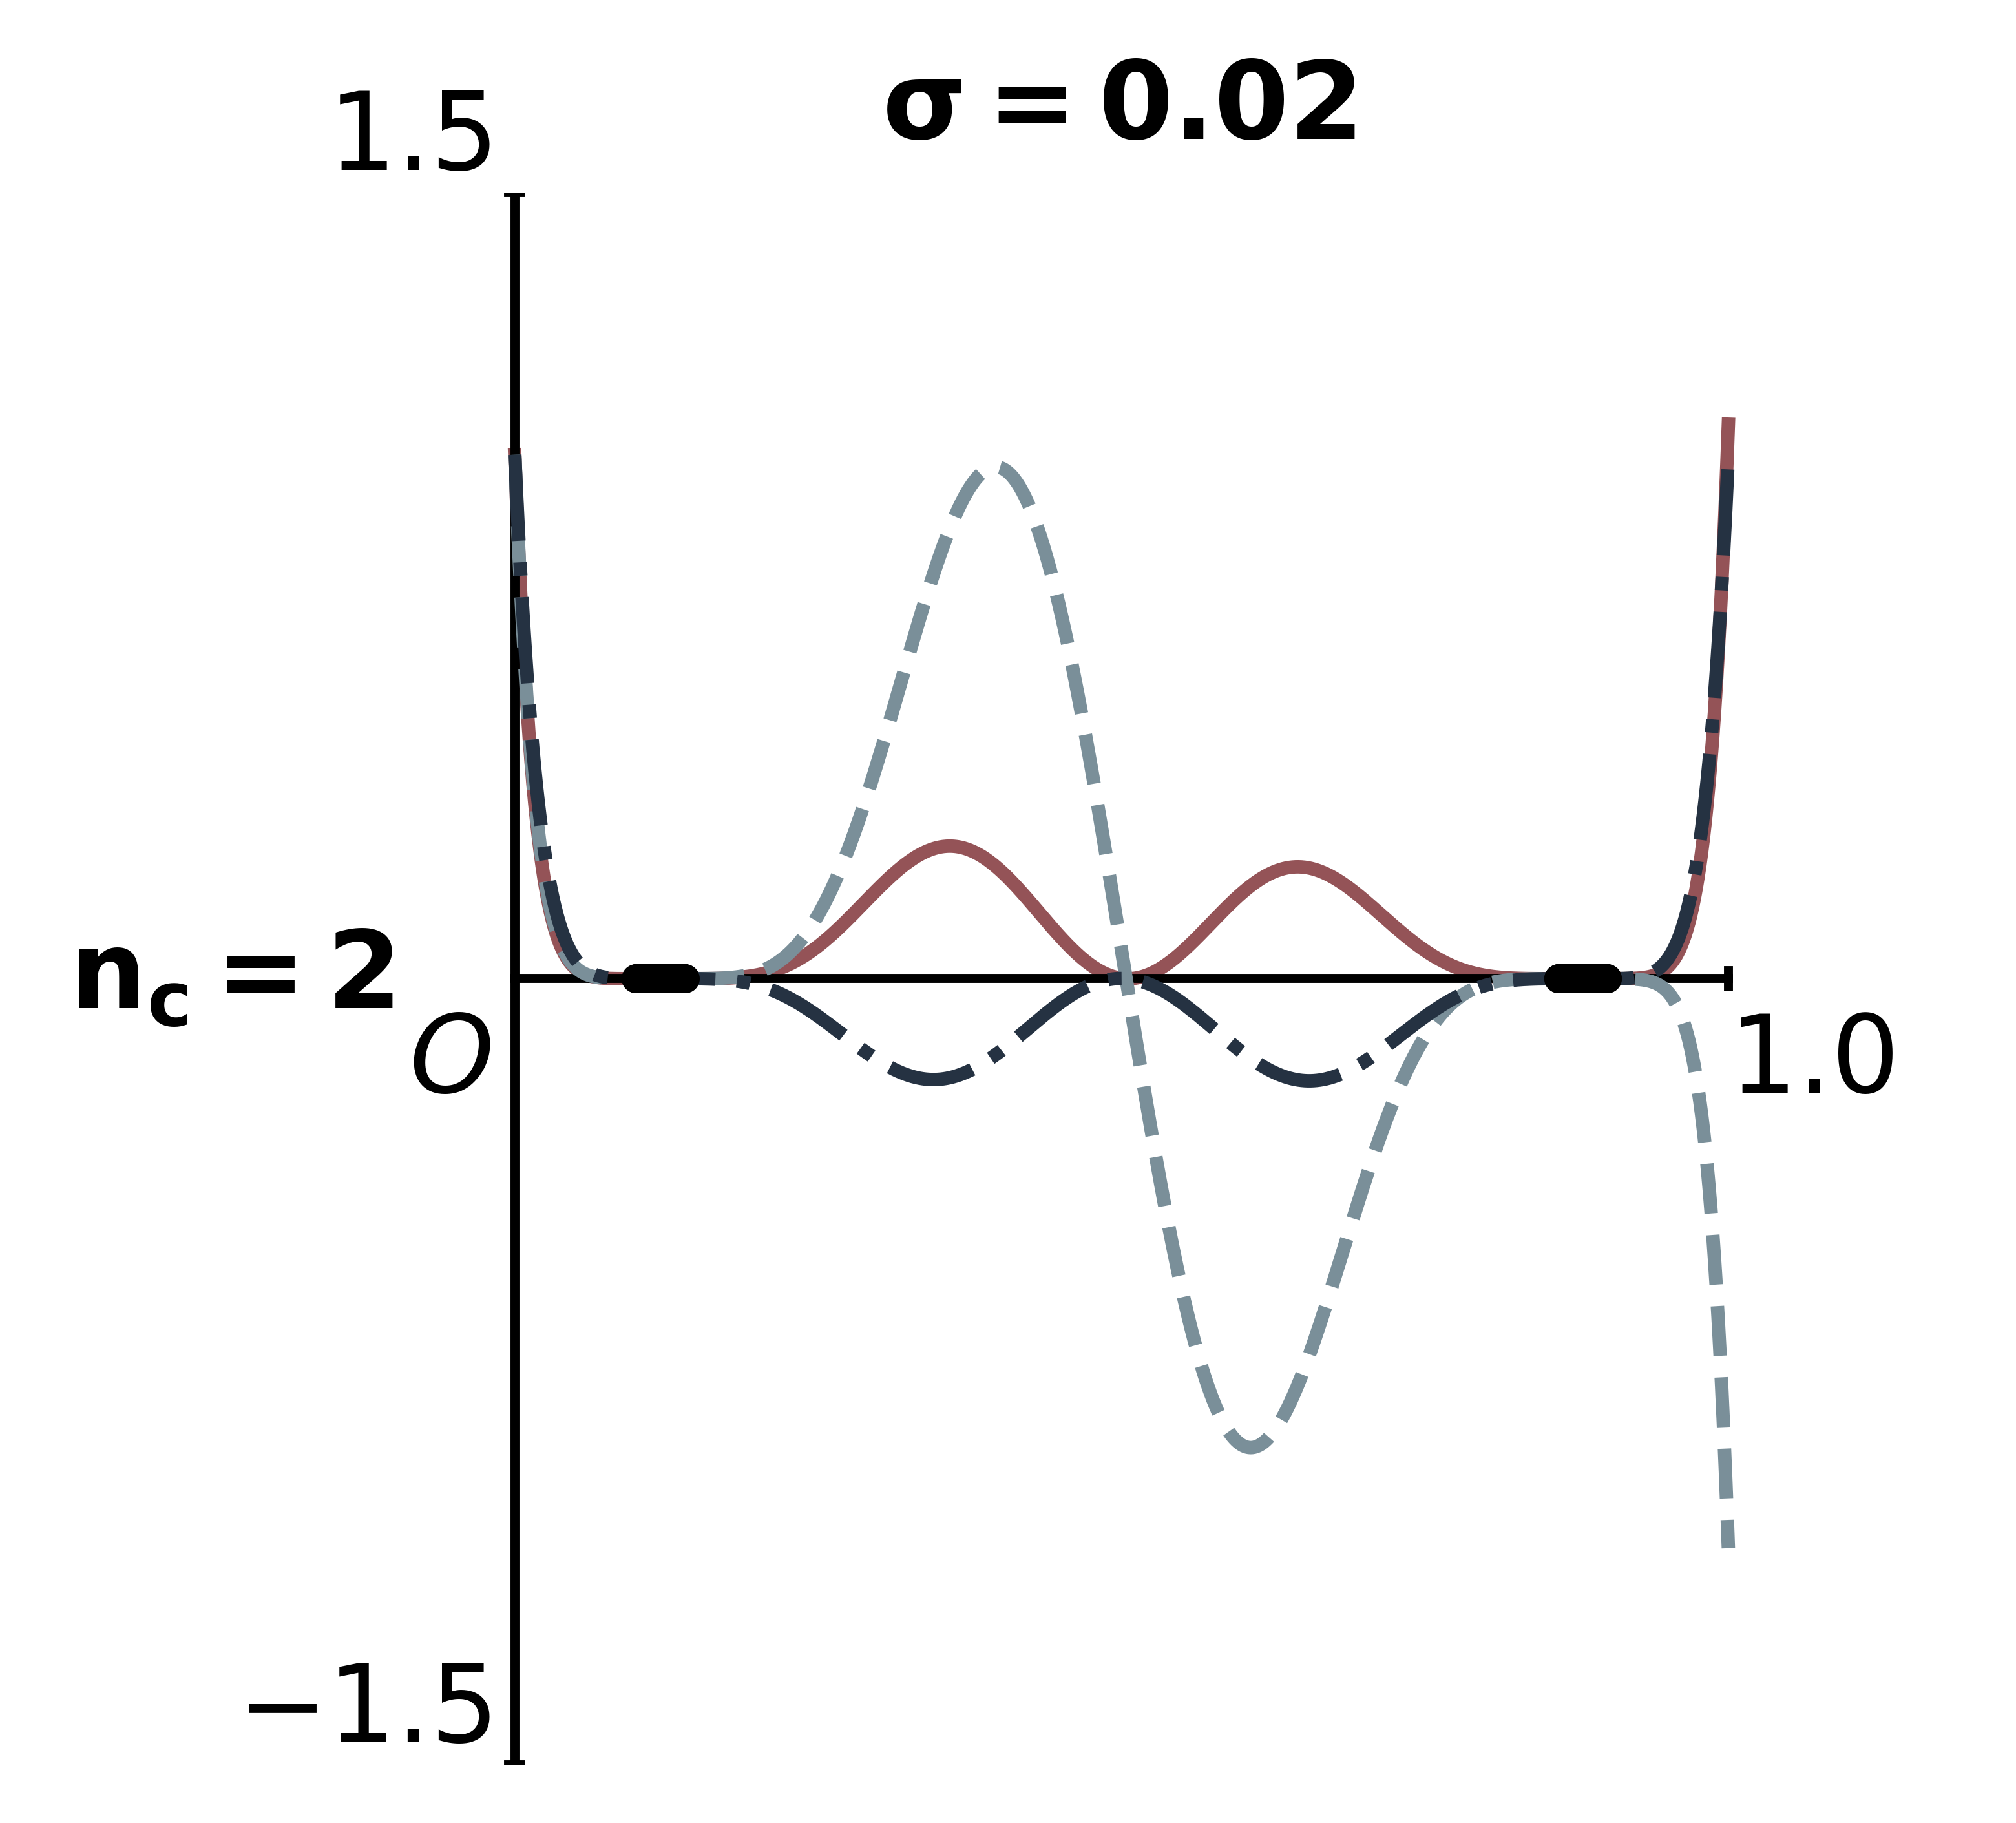
\includegraphics[width=0.4\paperwidth]{two_cluster_respoly.png}}

\institute[University]{
  \strut\llap{\inst{1}\,}Delft University of Technology
}
\date[EEMCS-DIAM-NA MSc. Thesis \monthyeardate]{EEMCS-DIAM Numerical Analysis MSc. Thesis Presentation, \monthyeardate}

% command for including images
\newcommand{\absimage}[4][0.5,0.5]{%
	\begin{textblock}{#3}%width
		[#1]% alignment anchor within image (centered by default)
		(#2)% position on the page (origin is top left)
		\includegraphics[width=#3\paperwidth]{#4}%
\end{textblock}}

\begin{document}

\titleframe

\begin{frame}[label=opening]{Darcy Problem}
    \frametitle{Opening}
    \framesubtitle{Darcy Problem}
\end{frame}

\begin{frame}[label=opening]{Conjugate Gradient Method}
    \frametitle{Opening}
    \framesubtitle{Conjugate Gradient Method}
\end{frame}

\begin{frame}[label=opening]{Condition Number}
    \frametitle{Opening}
    \framesubtitle{Condition Number}
\end{frame}

\begin{frame}[label=opening]{Preconditioners}
    \frametitle{Opening}
    \framesubtitle{Preconditioners}
\end{frame}

\begin{frame}[label=opening]{Research Gap}
    \frametitle{Opening}
    \framesubtitle{Research Gap}
\end{frame}

\begin{frame}[label=toc]{Structure}
    \frametitle{Structure}
    \begin{itemize}
        \item Introducing CG
        \item How Does CG Converge? The Role of Eigenvalues
        \item Preconditioning: Taming High-Contrast Problems
        \item High-contrast coefficients: split eigenspectrum
        \item Towards Sharper Iteration Bounds
        \item Multi-Cluster Spectra
        \item How Sharp Are the New Bounds?
        \item New Bounds in Practice: Using Ritz Values
        \item Conclusion: Key Takeaways \& Future Directions
    \end{itemize}
\end{frame}

\begin{comment}
Level 0: Opening (no header)
- Opening question: "What do X, Y, Z have in common?". (Show X, Y and Z with single picture slides and make sure to give short descriptions. Go quickly through the single-picture slides.)
- Answer: "They can all be modelled by a..." high-contrast diffusion problem for $u, u_D \in H^1(\Omega)$, $f\in L^2(\Omega)$ and $\mathcal{C}\in L^{\infty}(\Omega)$
    \begin{equation*}
        \begin{aligned}
            -\nabla\cdot\left(\mathcal{C}\nabla u\right) & = f \quad \text{in } \Omega           \\
            u                                            & = u_D \quad \text{on } \partial\Omega
        \end{aligned}
    \end{equation*}
- Understanding the problem: We need to find $u \in H^1(\Omega)$ such that the above equation holds.
- Briefly explain why discretization is necessary for PDEs, for non-experts.
- Linear system of equations $A\mathbf{u}=\mathbf{b}$
- We can compute approximations $\mathbf{u}_1, \mathbf{u}_2, \ldots$ efficiently using the CG method.
- Main R.Q.: "How can improve existing estimates on the total number of necessary CG iterations?"
- FEM discretization $\Omega\rightarrow\mathcal{T}$, $\nabla \rightarrow A$, $u\rightarrow\mathbf{u}$, $f\rightarrow\mathbf{b}$

Level 1: Introducing CG
- CG takes in initial guess $\mathbf{u}_0$ and provides updated solution $\mathbf{u}_k$ after $k$ iterations.
- Classical bound given relative error tolerance $\epsilon_m = \frac{\|\mathbf{e}_m\|_A}{\|\mathbf{e}_0\|_A} \leq \epsilon$ is
$\epsilon_m \leq 2\left(\frac{\sqrt{\kappa} - 1}{\sqrt{\kappa} + 1}\right)^{m} \longrightarrow m \leq \left\lfloor\frac{\sqrt{\kappa}}{2}\ln\left(\frac{2}{\epsilon}\right) + 1\right\rfloor = m_1(\kappa)$
- However $m_1$ can be too pessimistic for high-contrast problems. That is, $m \ll m_1$
- Restate R.Q.: "How do we improve/sharpen the classical bound $m_1$ for model problem?"

Level 2: How Does CG Converge? The Role of Eigenvalues
- When discussing eigenvalues, a simple visual or analogy could help non-mathematicians.
- Spectrum $\sigma(A) = \{\lambda_1, \ldots, \lambda_n\}$ and $\kappa(A) = \frac{\lambda_{\max}}{\lambda_{\min}}$
- CG solution given as $\mathbf{u}_m = \mathbf{u}_0 + q(A)\mathbf{r}_0$, with polynomial $q$ being the \textit{solution polynomial}.
- CG residual polynomial $r(\lambda) = 1 - \lambda q(\lambda)$
- Error expression $\epsilon_m = \frac{\|\mathbf{e}_m\|_A}{\|\mathbf{e}_0\|_A} < \min_{r \in \mathcal{P}_{m-1}, r(0) = 1} \max_{\lambda \in \sigma(A)} |r(\lambda)|$
- Animation: cg_residual_poly
- Loop through different randomized, clustered spectra, showing r_m for each.
- Show best and worst case scenario's for CG convergence
- Restate R.Q.: "How can we construct an CG iteration bound that accounts for the influence of the eigenvalue distribution?"

Level 3: Preconditioning: Taming High-Contrast Problems
- Why do we want to account for eigenvalue distribution? (practical motivation)
- High-contrast $C$ leads to spectral gap and $\kappa(A)\gg1$
- Clarify what "preconditioning" means in practical terms (e.g., analogy to making a problem easier to solve).
- Mathematically: transform $A\mathbf{u}=\mathbf{b}$ into $M^{-1}A\mathbf{u}=M^{-1}\mathbf{b}$, with preconditioner $M$. This leads to a reduced spectral gap and lower conditioner number. Then, apply CG as usual (now called Preconditioned CG or PCG)
- Show Filipe & Alexander's Research: they used three kinds of preconditioners $M_1, M_2, M_3$ and all had similar conditioner numbers and thereby similar upper bounds for their iteration number, $m_1(\kappa)$.
- However, on a sample problem PCG with $M_1,M_2$ needed significantly less iterations than PCG with $M_3$.
- Restate R.Q.: "How can we construct a CG iteration bound that can distinguish between different preconditioners with similar conditioner numbers?"

Level 4: Towards Sharper Iteration Bounds
- Recap: $\epsilon_m < \min_{r \in \mathcal{P}_{m-1}, r(0) = 1} \max_{\lambda \in \sigma(A)} |r(\lambda)| \leq \epsilon$
- Head-on strategy for a bound: try to find an $m^{\text{th}}$-order polynomial that satisfies the min-max problem.
- Classical bound invokes: optimal Chebyshev polynomial $r(\lambda) = \hat{C}_m$, under the assumption of a uniform interval of eigenvalues $\sigma(A) = [\lambda_{\min}, \lambda_{\max}]$ (inaccurate!).
- Simplest non-trivial case (one spectral gap): two disjoint clusters
- Axelsson, assume two uniform intervals and invoke $r(\lambda) = \hat{C}_{p}\hat{C}_{p-m}$
- Resulting two-cluster bound $m_2(\kappa, \kappa_l, \kappa_r)=\left\lfloor\frac{\sqrt{\kappa_r}}{2} \ln (2 / \epsilon)+\left(1+\frac{\sqrt{\kappa_r}}{2} \ln \left(\frac{4\kappa}{\kappa_l}\right)\right) p\right\rfloor$
- Restate R.Q.: "How can we construct an CG iteration bound that accounts for the influence of the eigenvalue distribution for general spectra?"

Note: The transition from classical bounds to multi-cluster bounds could be made more explicit—perhaps with a summary slide or visual.

Level 5: Multi-Cluster Spectra
- Depending on coefficient function and preconditioned systems we can have any number of clusters.
- Extend Axelsson idea: $r(\lambda) = \hat{C}^{(1)}_{p_1}\hat{C}^{(2)}_{p_2}\ldots\hat{C}^{(k)}_{p_k} = \prod_{i=1}^{k} \hat{C}^{(i)}_{p_i}$
- Multi-cluster bound: $p_i \leq \left\lceil\log_{f_i}{\frac{\epsilon}{2}} + \sum_{j=1}^{i-1} p_j\log_{f_i}\left(\frac{\zeta^{(j)}_2}{\zeta^{(i,j)}_1}\right)\right\rceil$ and $m_{N_{\text{cluster}}} = \sum_{i=1}^{N_{\text{cluster}}} p_i$, depends on the extremal eigenvalues of \textit{each cluster}
- We need a way of partitioning a given spectrum $\sigma(A)$ into $N_{\text{cluster}}$ clusters.
- Idea: simple, we split at the largest (relative) gap between subsequent eigenvalues, check if the two resulting clusters would give a sharper bound than just one uniform cluster, that is $m_2(\kappa, \kappa_l, \kappa_r) < m_1(\kappa)$. If so, we split the clusters and repeat the process for each created cluster. If not, we stop partitioning. In the process we keep track of all the extremal eigenvalues. After partitioning, we calculate $m_{N_{\text{cluster}}}$.
- Animation: cluster_partitioning, visualize above partitioning and subsequent calculation $m_{N_{\text{cluster}}}$.
- Restate R.Q.: "How much sharper is $m_{N_{\text{cluster}}}$ compared to $m_1(\kappa)$ for our model problem?"

Level 6: How Sharp Are the New Bounds?
- We implement the model problem with the two coefficient functions that Filipe and Alexander used and solve them using PCG with preconditioners $M_1, M_2, M_3$.
- First experiment: For each $\sigma(M_i^{-1}A)$, we compute $m_{N_{\text{cluster}}}$ and $m_1(\kappa)$ for comparison. As well as, $m_{N_{\text{tail-cluster}}}$, a variant of $m_{N_{\text{cluster}}}$ that can take in clusters as well as individual eigenvalues.
- Results: the new bounds are incredibly sharp as they are anywhere from 2 to 4 times as big as $m$. For comparison, $m_1$ is anywhere from 100 to 1000 times bigger than $m$, where the difference increases for spectra with larger spectral gaps
- Restate R.Q.: "How can we compute $m_{N_{\text{cluster}}}$ for our model problem in practice?"

Level 7: New Bounds in Practice: Using Ritz Values
- Problem: computing $m_{N_{\text{cluster}}}$ requires a good estimate of $\sigma(M_i^{-1}A)$.
- Luckily, PCG gives us exactly that, every iteration it produces a set of so-called Ritz values that is `close' to the true eigenvalue distribution. In particular, at the $k^{\text{th}}$ iteration, we get a set of $k$ Ritz values that we can use as an approximation of the full spectrum $\sigma(M_i^{-1}A)$.
- Second experiment, we use the Ritz values from the PCG iterations to compute $m_{N_{\text{cluster}}}$ and $m_1(\kappa)$ for our model problem and observe how good of an upper bound for $m$ we can obtain within the first 300 iterations.
- Results: For PCG with preconditioners $M_1, M_2$ (fast converging) $m_{N_{\text{cluster}}}$ gives sharp upper bounds for $m$ in all cases. However, for PCG with $M_3$ (slow converging) $m_{N_{\text{cluster}}}$ underestimates $m$ in some cases. This is because the Ritz values do not yet capture the full spectrum well enough within 300 iterations.
- Animation: ritz_value_migration

Level 8: Key Takeaways \& Future Directions
- The main goal of this thesis was to sharpen the CG iteration bound for high-contrast heterogeneous scalar-elliptic problems beyond the classical condition number-based bound. The derived multi-cluster and tail-cluster bounds offer a more nuanced and accurate picture of convergence behavior than the classical condition number-based bound, able to distinguish between preconditioners effectively.
- Though the utility of these bounds for early estimation depends on the specific coefficient function and preconditioner used.
- Future work:
- Should focus on applying the new bounds to a wider range of problems, including those with more complex high-contrast coefficients, finer mesh discretizations, different preconditioners, and other types of PDEs.
- research into the \textit{a priori}  estimation of the key spectral characteristics ($\kappa_l, \kappa_r, s$) is crucial to circumvent the dependency of the new bounds on the slowly converging Ritz values
- Closer: "Today we learned to not judge a preconditioner by its conditioner number. Instead, we learned to look at the richness contained within the preconditioned spectrum... today, we truly went \textit{beyond condition number}."
\end{comment}

\begin{frame}{Structure: Research Questions}
    \frametitle{Structure}
    \begin{itemize}
        \item {\color{tud grapefruit}Research Questions}
        \item Mathematical Background
        \item Related Work
        \item Preliminary Results
        \item Outlook
    \end{itemize}
\end{frame}

\begin{frame}[label=questions]{Research Questions: Main}
    \frametitle{Research Questions}
    \framesubtitle{Main Research Question}
    \vspace{0.2\pageheight}
    \begin{center}
    \textit{\textbf{How can we refine the CG iteration bound for Schwarz-preconditioned high-contrast heterogeneous elliptic problems beyond the classical condition number-based bound?}}
    \end{center}
\end{frame}

\begin{frame}[label=questions]{Research Questions: Sub}
    \frametitle{Research Questions}
    \framesubtitle{Subsidiary Research Questions}
    \setlength\itemindent{1in}
    \begin{itemize}
        \item[\textbf{Q1}] What other spectral characteristics like the condition number can we consider?
        \item[\textbf{Q2}] How to estimate the characteristics from \textbf{Q1}?
        \item[\textbf{Q3}] Given a toy eigenspectrum, how can we sharpen the CG iteration bound?
        \item[\textbf{Q4}] How does the sharpened bound from \textbf{Q3} compare to the classical CG bound?
        \item[\textbf{Q5}] How does the performance described in \textbf{Q4} depend on the characteristics found in \textbf{Q1}?
        \item[\textbf{Q6}] Can the sharpened bound from \textbf{Q3} distinguish between preconditioners? 
    \end{itemize}
\end{frame}

\chapter{Mathematical background}\label{ch:background}
In \cref{sec:cg_method} we discuss the classification of the CG method as both an error projection and a Krylov subspace method. We then derive the convergence rate of CG in \cref{sec:cg_convergence_rate}, as well as the influence of the eigenvalues of the system matrix $A$ on that rate in \cref{sec:cg_eigenvalue_distribution}. The latter is important, since it shows that the condition number $\kappa(A)$ is not the only factor influencing the convergence rate of CG. The first part ends with a brief review of the PCG method in \cref{sec:cg_preconditioning}. Then, the second part of this chapter \cref{sec:schwarz_methods} concerns the Schwarz methods, which are a class of domain decomposition methods. Schwarz methods can be used to construct preconditioners for use in PCG, even though these were originally devised as fixed point iteration methods for solving PDEs on complex domains. In \cref{sec:schwarz_convergence}, we also see some conditioner number estimates that are classically used to estimate the convergence rate of PCG.

\section{Conjugate gradient method}\label{sec:cg_method}
We seek to solve the linear system of equations $A\mathbf{u} = \mathbf{b}$, where $A$ is a symmetric positive definite (SPD) matrix. These properties of $A$ make the CG method particularly suitable for solving the system, as motivated in the \cref{ch:introduction}.

\subsection{Projection methods}
To further understand the CG method, we need to introduce the class of \textit{projection methods}, which given some initial guess $\mathbf{u}_0$ find an approximation $\mathbf{u}_{\text{new}}$ to the solution of the linear system $A\mathbf{u} = \mathbf{b}$ in a \textit{constrained subspace} $\mathcal{L}\subset\mathbb{R}^n$ using a \textit{correction vector} $\mathbf{c}$ in another subspace $\mathcal{K}\subset\mathbb{R}^n$. That is, projection methods solve the following problem \cite[Equation 5.3]{iter_method_saad}
\[
  \text{Find } \mathbf{u}_{\text{new}} = \mathbf{u}_0 + \mathbf{c} \in \mathbf{u}_0 + \mathcal{K} \text{ such that } \mathbf{r}_{\text{new}} =  A\mathbf{u}_{\text{new}} - \mathbf{b} = \mathbf{r}_0 - A\mathbf{c} \perp \mathcal{L}.
\]
In doing so, projection methods perform a \textit{projection step}, visualized in \cref{fig:projection_method}.
\begin{figure}[H]
  \centering
  \begin{tikzpicture}
    % Origin
    \coordinate (O) at (0,0);
    \node[below=0.5pt of O] {O};

    % Plane L
    \coordinate (L_bottom_left) at (-3,-1);
    \coordinate (L_bottom_right) at (1,-1);
    \coordinate (slant_vec) at (2, 2); % Slant for perspective (top edge shifted left and up)
    \coordinate (L_top_right) at ($(L_bottom_right) + (slant_vec)$);
    \coordinate (L_top_left) at ($(L_bottom_left) + (slant_vec)$);

    \draw[thick] (L_bottom_left) -- (L_bottom_right) -- (L_top_right) -- (L_top_left) -- cycle;
    \node at ($(L_top_right) + (-0.6, -0.25)$) {$\mathcal{L}$}; % Label for L

    % Vector definitions
    \coordinate (Rnew_tip) at (0, 2.4); % Tip of r_new
    \coordinate (Ac_vec_val) at (1.6, 0); % Vector A*c (horizontal)
    \coordinate (R0_tip) at ($(Rnew_tip) + (Ac_vec_val)$); % Tip of r_0

    % Draw vectors and their labels
    \draw[-{Latex[length=2mm, width=1.5mm]}] (O) -- (Rnew_tip) node[below left=1pt and 1pt] {$\mathbf{r}_{\text{new}}$};
    \draw[-{Latex[length=2mm, width=1.5mm]}] (Rnew_tip) -- (R0_tip) node[midway, above=.5pt] {$A\mathbf{c}$};
    \draw[-{Latex[length=2mm, width=1.5mm]}] (O) -- (R0_tip) node[below left=18.5pt and .5pt] {$\mathbf{r}_{0}$};

    % Right angle symbol at O
    \def\rasize{0.25} % Size of the right angle symbol
    \coordinate (RA_up_on_rnew) at (0, \rasize); % Point on r_new from O
    \coordinate (RA_plane_line) at (-\rasize, 0); % Point on plane's front edge from O
    
    \draw[thin] (RA_up_on_rnew) -- (-\rasize,\rasize) -- (RA_plane_line); % The two lines forming the angle
    \draw[thick] (O) -- ($1.2*(RA_plane_line)$); % The line from O to the plane
\end{tikzpicture}
  \caption{Visualization of projection method, based on \cite[Figure 5.1]{iter_method_saad}. The projection method finds the solution $\mathbf{u}_{\text{new}}$ in the affine subspace $\mathbf{u}_0 + \mathcal{K}$, such that the new residual $\mathbf{r}_{\text{new}}$ is orthogonal to the constraint subspace $\mathcal{L}$.}
  \label{fig:projection_method}
\end{figure}

\subsubsection{Error projection methods}
The subclass of \textit{error projection methods} defined by \cref{def:error_projection_method} sets $\mathcal{K} = \mathcal{L}$.
\begin{fancydef}{Error projection method}{error_projection_method}
  To perform an error projection step, find $\mathbf{u}_{\text{new}} = \mathbf{u}_0 + \mathbf{c} \in \mathbf{u}_0 + \mathcal{K}$ such that
  \begin{equation}
    (\mathbf{r}_0 - A\mathbf{c}, w) = 0 \quad \forall w \in \mathcal{K},
    \label{eq:orthogonality_condition}
  \end{equation}
  where $(\cdot,\cdot)$ is an inner product on $\mathcal{K}$. Let $V = [\mathbf{v}_1, \mathbf{v}_2, \dots, \mathbf{v}_m]$ be a matrix whose columns span $\mathcal{K}$, then one error projection step is given by
  \begin{align*}
    \mathbf{u}_{\text{new}} & = \mathbf{u}_0 + V \mathbf{v} \\
    V^TAV\mathbf{v}         & = V^T\mathbf{r}_0,
  \end{align*}
\end{fancydef}
Error projection methods owe their name to the following central \cref{th:error_projection_method}.
\begin{fancyth}{Error minimization in $A$-norm}{error_projection_method}
  Given a linear system $A\mathbf{u} = \mathbf{b}$ with $A$ SPD and solution $\mathbf{u}^{*}$. Define the errors $\mathbf{e}_0 = \mathbf{u}^{*} - \mathbf{u}_0$ and $\mathbf{e}_{\text{new}} = \mathbf{u}^{*} - \mathbf{u}_{\text{new}}$. Then, an error projection step minimizes the $A$-norm of the error in the affine subspace $\mathbf{u}_0 + \mathcal{K}$.
\end{fancyth}
\begin{proof}
  We have
  \begin{align*}
    A\mathbf{e}_{\text{new}} & = A(\mathbf{e}_0 - \mathbf{c})                  \\
                             & = A(\mathbf{u}^{*} - \mathbf{u}_0 - \mathbf{c}) \\
                             & = \mathbf{r}_0 - A\mathbf{c}
  \end{align*}
  Hence, the orthogonality condition in \cref{eq:orthogonality_condition} can be written as
  \[
    (A\mathbf{e}_{\text{new}}, w) = (\mathbf{e}_0 - \mathbf{c}, w)_{A} = 0, \quad \forall w \in \mathcal{K}.
  \]
  In other words, the correction vector $\mathbf{c}$ is the $A$-orthogonal projection of the error $\mathbf{e}_0$ onto $\mathcal{K}$. Therefore, there exists a projection operator $P_{\mathcal{K}}^{A}$ such that $\mathbf{c} = P_{\mathcal{K}}^{A}\mathbf{e}_0$ and we can write
  \[
    \mathbf{e}_{\text{new}} = (I - P_{\mathcal{K}}^{A}) \mathbf{e}_0.
  \]
  Moreover, we have using symmetry and positive definiteness of $A$ that we can define the $A$-norm $\|\cdot\|_A$. Then, using the $A$-orthogonality between the error $\mathbf{e}_{\text{new}}$ and the correction $P_{\mathcal{K}}^{A}\mathbf{e}_0$, we get
  \begin{align*}
    \|\mathbf{e}_{0}\|_A^2 & = \|\mathbf{e}_{\text{new}}\|_A^2 + \|P_{\mathcal{K}}^{A}\mathbf{e}_0\|_A^2 \\
                           & \geq \|\mathbf{e}_{\text{new}}\|_A^2,
  \end{align*}
  which shows that the new error is smaller than the previous error in the $A$-norm. To show that the error projection step minimizes the $A$-norm of the error in the affine subspace $\mathbf{u}_0 + \mathcal{K}$, we let $\mathbf{x}\in\mathbb{R}^n$ and $\mathbf{y} \in \mathbf{u}_0 + \mathcal{K}$ be arbitrary, then using that $P_{\mathcal{K}}^{A}\mathbf{x} - \mathbf{y} \in \mathbf{u}_0 + \mathcal{K}$ we get
  \begin{align*}
    \|\mathbf{x} - \mathbf{y}\|_A^2 & = \|\mathbf{x} - P_{\mathcal{K}}^{A}\mathbf{x} + P_{\mathcal{K}}^{A}\mathbf{x} - \mathbf{y} \|_A^2        \\
                                    & = \|\mathbf{x} - P_{\mathcal{K}}^{A}\mathbf{x}\|_A^2 + \|P_{\mathcal{K}}^{A}\mathbf{x} - \mathbf{y}\|_A^2 \\
                                    & \geq \|\mathbf{x} - P_{\mathcal{K}}^{A}\mathbf{x}\|_A^2,
  \end{align*}
  which yields that \cite[Theorem 1.38]{iter_method_saad}
  \begin{equation}
    \min_{\mathbf{y} \in \mathbf{u}_0 + \mathcal{K}} \|\mathbf{x} - \mathbf{y}\|_A = \|\mathbf{x} - P_{\mathcal{K}}^{A}\mathbf{x}\|_A.
    \label{eq:projection_minimization}
  \end{equation}
  Now, substituting $\mathbf{x} = \mathbf{e}_0$ and $\mathbf{y} = \mathbf{c}$ into \cref{eq:projection_minimization}, we again find $\mathbf{c} = P_{\mathcal{K}}^{A}\mathbf{e}_0$, giving the desired result.
\end{proof}

\subsubsection{General algorithm for error projection methods}
By performing multiple (error) projection steps we obtain a sequence of approximations $\{\mathbf{u}_0, \mathbf{u}_1, \dots, \mathbf{u}_m\}$ to exact the solution $\mathbf{u}^*$ of the linear system $A\mathbf{u} = \mathbf{b}$. \cref{th:error_projection_method} ensures that each approximate solution $\mathbf{u}_j$ is closer to the exact solution $\mathbf{u}^*$ than the previous one $\mathbf{u}_{j-1}$. This idea forms the basis for a general error projection method and results in \cref{alg:error_projection_method}
\begin{algorithm}[H]
  \caption{Prototype error projection method \cite[Algorithm 5.1]{iter_method_saad}}
  \begin{algorithmic}
    \State Set $\mathbf{u} = \mathbf{u}_0$
    \While{$\mathbf{u}$ is not converged}
    \State Choose basis $V$ of $\mathcal{K}=\mathcal{L}$
    \State $\mathbf{r} = \mathbf{b} - A \mathbf{u}$
    \State $\mathbf{c} = (V^TAV)^{-1}V^T\mathbf{r}$
    \State $\mathbf{u} = \mathbf{u} + V\mathbf{c}$
    \EndWhile
  \end{algorithmic}
  \label{alg:error_projection_method}
\end{algorithm}
Projection methods differ in their choice of the spaces $\mathcal{K}$ and $\mathcal{L}$ as well as in how they obtain the basis $V$ of $\mathcal{K}$, as well as the so-called \textit{Hessenberg matrix} defined in \cref{def:hessenberg_matrix}.
\begin{fancydef}{Hessenberg matrix}{hessenberg_matrix}
  The Hessenberg matrix $H$ is defined as the matrix $H = V^TAV$, where $V$ is a matrix whose columns span the subspace $\mathcal{K}$.
\end{fancydef}

\subsubsection{Krylov subspace methods}
Krylov subspace methods form yet another subclass of projection methods and are defined by their choice of the space $\mathcal{K}$. Namely,
\begin{equation}
  \mathcal{K}_m(A_0, \mathbf{r}_0) = \text{span}\{\mathbf{r}_0, A\mathbf{r}_0, A^2\mathbf{r}_0, \dots, A^{m-1}\mathbf{r}_0\},
  \label{eq:cg_krylov_space}
\end{equation}
or $\mathcal{K}_m$ as a shorthand.
\begin{definition}
  The grade of a vector $\mathbf{v}$ with respect to a matrix $A$ is the lowest degree of the polynomial $q$ such that $q(A)\mathbf{v} = 0$.
  \label{def:cg_grade}
\end{definition}
Consequently,
\begin{theorem}
  The Krylov subspace $\mathcal{K}_m$ is of dimension $m$ if and only if the grade $\mu$ of $\mathbf{v}$ with respect to $A$ is not less than $m$ \cite[proposition 6.2]{iter_method_saad},
  \begin{equation*}
    \dim(\mathcal{K}_m) = m \iff \mu \geq m,
  \end{equation*}
  such that
  \begin{equation}
    \dim(\mathcal{K}_m) = \min \{m, \textrm{grade}(\mathbf{v})\}.
    \label{eq:cg_krylov_dimension}
  \end{equation}
  \label{th:cg_krylov_dimension}
\end{theorem}

\begin{definition}
  The action of a matrix $A$ can be thought of as a mapping
  \begin{equation*}
    \mathbb{R}^n \rightarrow \mathbb{R}^n: v \mapsto A v
  \end{equation*}
  Thus the domain and codomain of $A$ are $\mathbb{R}^n$. Let $X \subset \mathbb{R}^n$, we can consider the map
  \begin{equation*}
    X \rightarrow \mathbb{R}^n: v \mapsto A v
  \end{equation*}
  instead. The only difference from $A$ is that the domain is $X$. This map is defined as the restriction $A_{\left.\right|_X}$ of $A$ to $X$.
\end{definition}

\begin{definition}
  Let $Q$ be a projector onto the subspace $X$. Then the section of the operator $A$ onto $X$ is defined as $QA_{\left.\right|_X}$.
\end{definition}

\begin{theorem}
  Let $Q_m$ be any projector onto $\mathcal{K}_m$ and let $A_m$ be the section of $A$ to $\mathcal{K}_m$, that is, $A_m=Q_m A_{\left.\right|\mathcal{K}_m}$. Then for any polynomial $q$ of degree not exceeding $m-1$ \cite[proposition 6.3]{iter_method_saad},
  \begin{equation*}
    q(A) v=q\left(A_m\right) v
  \end{equation*}
  and for any polynomial of degree $\leq m$,
  \begin{equation*}
    Q_m q(A) v=q\left(A_m\right) v
  \end{equation*}
\end{theorem}

\subsection{CG algorithm}
The CG method exists in the intersection of error projection methods and Krylov subspace methods, as it is a projection method with the choice $\mathcal{L} = \mathcal{K} = \mathcal{K}_m$. We can derive the CG method starting from Arnoldi's method, see \cref{alg:arnoldi_linear_systems}. Arnoldi's method is much like \cref{alg:error_projection_method} in that it uses a Gramm-Schmidt orthogonalization procedure to obtain the basis $V$ of the Krylov subspace $\mathcal{K}_m$ and a projection step to update the solution. Where Arnoldi's method is applicable to non-symmetric matrices by performing a full orthogonalization step, CG leverages the symmetry of $A$ by doing a partial orthogonalization step. The latter is possible, since the CG method only needs to maintain the orthogonality of the residuals $\mathbf{r}_j$ with respect to the previous residuals $\mathbf{r}_{j-1}$ and not with respect to all previous residuals $\mathbf{r}_{j-2}, \dots, \mathbf{r}_0$. The full derivation is discussed in the Appendix, \cref{sec:cg_derivation} and results in \cref{alg:cg}.
\begin{algorithm}[H]
  \caption{Conjugate Gradient Method}
  \begin{algorithmic}
    \State $\mathbf{r}_0 = \mathbf{b} - A\mathbf{u}_0$, $\mathbf{p}_0 = \mathbf{r}_0$, $\beta_0 = 0$
    \For{$j = 0, 1, 2, \dots, m$}
    \State $\alpha_j = (\mathbf{r}_j, \mathbf{r}_j) / (A \mathbf{p}_j, \mathbf{p}_j)$
    \State $\mathbf{u}_{j+1} = \mathbf{u}_j + \alpha_j \mathbf{p}_j$
    \State $\mathbf{r}_{j+1} = \mathbf{r}_j - \alpha_j A \mathbf{p}_j$
    \State $\beta_j = (\mathbf{r}_{j+1}, \mathbf{r}_{j+1}) / (\mathbf{r}_j, \mathbf{r}_j)$
    \State $\mathbf{p}_{j+1} = \mathbf{r}_{j+1} + \beta_j \mathbf{p}_j$
    \EndFor
  \end{algorithmic}
  \label{alg:cg}
\end{algorithm}
A crucial property of the approximate solution that \cref{alg:cg} produces is given in \cref{th:cg_approximate_solution}
\begin{fancyth}{CG approximate solution}{cg_approximate_solution}
  The approximate solution at the $m^{\text{th}}$ iteration is given by
  \begin{equation}
    \mathbf{u}_m = \mathbf{u}_0 + \sum_{i=0}^{m-1} c_i A^i \mathbf{r}_0 = \mathbf{u}_0 + q_{m-1}(A)\mathbf{r}_0,
    \label{eq:cg_approximate_solution}
  \end{equation}
  where $q_{m-1}(A)$ is the solution polynomial of degree $m-1$ in $A$.
\end{fancyth}
\begin{proof}
  The CG method is a projection method with the choice $\mathcal{L} = \mathcal{K} = \mathcal{K}_m$. Hence, the approximate solution $\mathbf{u}_m$ is an element of the affine Krylov subspace $\mathbf{u}_0 + \mathcal{K}_m(A, \mathbf{r}_0)$, see \cref{def:error_projection_method}. The result follows from the fact that the Krylov subspace $\mathcal{K}_m(A, \mathbf{r}_0)$ is spanned by the vectors $\{\mathbf{r}_0, A\mathbf{r}_0, A^2\mathbf{r}_0, \dots, A^{m-1}\mathbf{r}_0\}$ and that the approximate solution $\mathbf{u}_m$ is a linear combination of these vectors. The coefficients of this linear combination are given by the \textit{CG solution coefficients} $c_i$.
\end{proof}

\subsection{CG convergence}\label{sec:cg_convergence}
We derive a general bound for the error of the CG method in
\begin{fancyth}{CG general error bound}{cg_error_bound}
  Suppose we apply the CG method to the linear system $A\mathbf{u} = \mathbf{b}$ with $A$ SPD and the exact solution $\mathbf{u}^*$. Then, the error of the $m^{\text{th}}$ iterate $\mathbf{e}_m = \mathbf{u}^* - \mathbf{u}_m$ is bounded as
  \begin{equation}
    ||\mathbf{e}_m||_A < \min_{r \in \mathcal{P}_{m-1}, r(0) = 1} \max_{\lambda \in \sigma(A)} |r(\lambda)| ||\mathbf{e}_0||_A.
    \label{eq:cg_error_bound}
  \end{equation}
\end{fancyth}
\begin{proof}
  Combining the results of \cref{th:error_projection_method} and \cref{th:cg_approximate_solution} we get that the error of the $m^{\text{th}}$ iterate of the CG algorithm $\mathbf{e}_m = \mathbf{u}^* - \mathbf{u}_m$ satisfies
  \begin{equation}
    \|\mathbf{e}_m\|_A = \|(I - Aq_{m-1}(A))\mathbf{e}_0\|_A = \min_{q \in \mathcal{P}_{m-1}}\|(I - Aq(A))\mathbf{e}_0\|_A = \min_{r \in \mathcal{P}_{m}, r(0) = 1}\|r(A)\mathbf{e}_0\|_A,
    \label{eq:cg_error}
  \end{equation}
  where $r_m(A) = I - Aq_{m-1}(A)$ is the \textit{residual polynomial}. The right-hand side of \cref{eq:cg_error} can be further bounded by letting $\lambda_i, \xi_i$ be the eigenvalues of $A$ and the components of $\mathbf{e}_0$ in the eigenbasis of $A$, respectively. Then
  \[
    ||r(A)\mathbf{e}_0||_A = \sqrt{\sum_{i=1}^n |r(\lambda_i)|^2 |\xi_i|^2} \leq \max_{\lambda \in \sigma(A)} |r(\lambda)| ||\mathbf{e}_0||_A,
  \]
  which gives the desired result.
\end{proof}

\subsubsection{Convergence criteria}\label{sec:cg_convergence_criteria}
We say that the CG method \textit{converges} to a user-defined, absolute tolerance $\tilde{\epsilon}$ if the error of the $m^{\text{th}}$ iterate $\mathbf{e}_m$ satisfies
\[
  \|\mathbf{e}_m\|_A \leq \tilde{\epsilon}.
\]
Now, \cref{th:cg_error_bound} allows us to define a criterion based on a \textit{relative tolerance} $\epsilon$, see \cref{def:cg_convergence_criterion}
\begin{fancydef}{Convergence criterion}{cg_convergence_criterion}
  The CG method is said to have \textit{converged} to a user-defined, relative tolerance $\epsilon$ if
  \begin{equation*}
    \frac{\|\mathbf{e}_m\|_A}{\|\mathbf{e}_0\|_A} \leq \epsilon,
  \end{equation*}
  which according to \cref{th:cg_error_bound} is satisfied when
  \begin{equation}
    \min_{r \in \mathcal{P}_{m-1}, r(0) = 1} \max_{\lambda \in \sigma(A)} |r(\lambda)| \leq \epsilon.
    \label{eq:cg_convergence_criterion}
  \end{equation}
\end{fancydef}
However, the criterion from \cref{def:cg_convergence_criterion} is not usable a stopping criterion during CG iterations, since it involves the usually unknown error $\mathbf{e}$. Luckily, \cref{th:residual_convergence_criterion} shows how we can relate the ratio of $A$-norms of the error to a similar ratio of the 2-norms of the residuals.
\begin{fancyth}{Residual convergence criterion}{residual_convergence_criterion}
  The CG method has converged to a user-defined, relative tolerance $\epsilon$ in the sense of \cref{def:cg_convergence_criterion} if
  \begin{equation}
    \frac{\|\mathbf{r}_m\|_2}{\|\mathbf{r}_0\|_2} \leq \frac{\epsilon}{\sqrt{\kappa}},
    \label{eq:residual_convergence_criterion}
  \end{equation}
  where $\kappa = \frac{\lambda_{\text{max}}}{\lambda_{\text{min}}}$ is the condition number of $A$.
\end{fancyth}
\begin{proof}
  We have for $i=0,m$ that
  \[
    \mathbf{e}_i = A^{-1}\mathbf{b} - \mathbf{u}_i = A^{-1}(\mathbf{b} - A\mathbf{u}_i) = A^{-1}\mathbf{r}_i.
  \]
  Therefore, we can write
  \[
    \frac{\|\mathbf{e}_m\|_A}{\|\mathbf{e}_0\|_A} = \frac{\mathbf{r}_0^TA^{-T}\mathbf{r}_m}{\mathbf{r}_0^TA^{-T}\mathbf{r}_0} = \frac{\|\mathbf{r}_m\|_{A^{-1}}}{\|\mathbf{r}_0\|_{A^{-1}}},
  \]
  where the last equality follows as $A^{-1}$ is SPD. Now, by \cref{th:rayleigh_quotient_bound} and using that the eigenvalues of $A^{-1}$ are the inverses of the eigenvalues of $A$, we can bound the $A^{-1}$-norm of the residuals as
  \[
    \|\mathbf{r}_m\|_{A^{-1}}  \leq \frac{1}{\sqrt{\lambda_{\text{min}}}} \|\mathbf{r}_m\|_2,
  \]
  and
  \[
    \|\mathbf{r}_0\|_{A^{-1}} \geq \frac{1}{\sqrt{\lambda_{\text{max}}}} \|\mathbf{r}_0\|_2.
  \]
  Hence, we can write
  \[
    \frac{\|\mathbf{e}_m\|_A}{\|\mathbf{e}_0\|_A} \leq \sqrt{\kappa} \frac{\|\mathbf{r}_m\|_2}{\|\mathbf{r}_0\|_2}.
  \]
  To conclude, if we perform the CG method until the convergence criterion \cref{eq:residual_convergence_criterion} is satisfied, we have
  \[
    \frac{\|\mathbf{e}_m\|_A}{\|\mathbf{e}_0\|_A} \leq \sqrt{\kappa} \frac{\|\mathbf{r}_m\|_2}{\|\mathbf{r}_0\|_2} \leq \epsilon,
  \]
  which gives the desired result.
\end{proof}
An important conclusion to draw from \cref{th:residual_convergence_criterion} is that if we set some relative tolerance for the residuals $\epsilon_r$ such that we stop iterating when
\begin{equation}
  \frac{\|\mathbf{r}_m\|_2}{\|\mathbf{r}_0\|_2} \leq \epsilon_r,
  \label{eq:residual_convergence_criterion_r}
\end{equation}
then we get that the CG method has converged to a relative error tolerance $\epsilon$ given by
\[
  \frac{\|\mathbf{e}_m\|_A}{\|\mathbf{e}_0\|_A} \leq \epsilon = \frac{\epsilon_r}{\sqrt{\kappa}}.
\]
This means that the CG method converges to a relative tolerance $\epsilon$ that is smaller than the relative tolerance of the residuals $\epsilon_r$ by a factor of $\sqrt{\kappa}$. On the one hand, this allows us to set a convergence criterion based on the residuals, which can actually be computed during CG iterations, as is the point of \cref{th:residual_convergence_criterion}. On the other hand, the convergence criterion based on the residuals is also pessimistic by the same factor of $\sqrt{\kappa}$. In other words, the CG method performs more iterations to converge to a stricter tolerance than the user-defined tolerance $\epsilon_r$.

Moreover, using \cref{th:rayleigh_quotient_bound} we can also bound the absolute error tolerance $\tilde{\epsilon}$ of the CG method in terms of the initial residual. That is, suppose we set $\epsilon_r$ as a convergence criterion, then we get
\begin{equation}
  \tilde{\epsilon} \leq \frac{\epsilon_r}{\sqrt{\kappa}}\|\mathbf{e}_0\|_A = \frac{\epsilon_r}{\sqrt{\kappa}}\|\mathbf{r}_0\|_{A^{-1}} \leq \frac{\epsilon_r}{\sqrt{\lambda_{\text{max}}}}\|\mathbf{r}_0\|_2.
  \label{eq:cg_absolute_error_bound_r}
\end{equation}

From \cref{th:residual_convergence_criterion} and choosing $\mathbf{u}_0 = \mathbf{0}\in\mathbb{R}^n$, we can derive a commonly implemented convergence criterion
\begin{equation}
  \frac{\|\mathbf{r}_m\|_2}{\|\mathbf{b}\|_2} \leq \epsilon_b.
  \label{eq:residual_convergence_criterion_b}
\end{equation}
In this case, the relative error tolerance $\epsilon$ achieved by the CG method in the sense of \cref{def:cg_convergence_criterion} still depends on the initial guess. Suppose, we choose a `good' initial guess such that $\|\mathbf{r}_0\|_2 \leq \|\mathbf{b}\|_2$, then
\[
  \frac{\|\mathbf{r}_m\|_2}{\|\mathbf{b}\|_2} \leq \frac{\|\mathbf{r}_m\|_2}{\|\mathbf{r}_0\|_2},
\]
which means \cref{eq:residual_convergence_criterion_b} is more optimistic than \cref{eq:residual_convergence_criterion_r}, requiring less CG iterations before it is satisfied. However, if we choose a `bad' initial guess such that $\|\mathbf{r}_0\|_2 \geq \|\mathbf{b}\|_2$, then \cref{eq:residual_convergence_criterion_b} is more pessimistic than \cref{eq:residual_convergence_criterion_r} and will require more CG iterations before it is satisfied. For a good (bad) initial guess we therefore achieve a relative error tolerance larger (smaller) than $\frac{\epsilon_b}{\sqrt{\kappa}}$. In regard to the absolute error tolerance $\tilde{\epsilon}$, we can write using \cref{th:rayleigh_quotient_bound} that
\begin{enumerate}
  \item[\textbf{good initial guess}] $\tilde{\epsilon} \geq \frac{\epsilon_b}{\sqrt{\kappa}}\|\mathbf{e}_0\|_A = \frac{\epsilon_b}{\sqrt{\kappa}}\|\mathbf{r}_0\|_{A^{-1}} \geq \frac{\sqrt{\lambda_{\text{min}}}}{\lambda_{\text{max}}}\epsilon_b\|\mathbf{r}_0\|_2\geq \frac{\sqrt{\lambda_{\text{min}}}}{\lambda_{\text{max}}}\epsilon_b\|\mathbf{b}\|_2$,
  \item[\textbf{bad initial guess}] $\tilde{\epsilon} \leq \frac{\epsilon_b}{\sqrt{\kappa}}\|\mathbf{e}_0\|_A = \frac{\epsilon_b}{\sqrt{\kappa}}\|\mathbf{r}_0\|_{A^{-1}} \leq \frac{\lambda_{\text{min}}}{\sqrt{\lambda_{\text{max}}}}\epsilon_b\|\mathbf{r}_0\|_2 \leq \frac{\lambda_{\text{min}}}{\sqrt{\lambda_{\text{max}}}}\epsilon_b\|\mathbf{b}\|_2$.
\end{enumerate}
In other words, when we use \cref{eq:residual_convergence_criterion_b} as a convergence criterion, the absolute error tolerance we achieve satisfies
\begin{equation}
  \frac{\sqrt{\lambda_{\text{min}}}}{\lambda_{\text{max}}}\epsilon_b\|\mathbf{b}\|_2 \leq \tilde{\epsilon} \leq \frac{\lambda_{\text{min}}}{\sqrt{\lambda_{\text{max}}}}\epsilon_b\|\mathbf{b}\|_2.
  \label{eq:cg_absolute_error_bound_b}
\end{equation}

Comparing \cref{eq:cg_absolute_error_bound_r} and \cref{eq:cg_absolute_error_bound_b} we gain the insight that when
\[
  \|\mathbf{r}_0\|_2 < \frac{\epsilon_b}{\epsilon_r\sqrt{\kappa}}\|\mathbf{b}\|_2,
\]
using convergence criterion \cref{eq:residual_convergence_criterion} is guaranteed to give a more accurate result than \cref{eq:residual_convergence_criterion_b}. On the other hand, if $\|\mathbf{r}_0\|_2$ is larger, then it might be better to use \cref{eq:residual_convergence_criterion_b} as a convergence criterion. In practice, criterion \cref{eq:residual_convergence_criterion_b} is used, since its accuracy bound in \cref{eq:cg_absolute_error_bound_b} holds, independent of initial guesses.

\subsubsection{Convergence rate}
Next to convergence criteria based on residuals, we can also try to find a solution to the minimization problem in \cref{eq:residual_convergence_criterion}, which gives us an expected convergence rate. Under the assumption of a uniform distribution of the eigenvalues of $A$, we can further bound the error of the $m^{\text{th}}$ iterate of the CG algorithm by a Chebyshev polynomial. This is done in \cref{th:cg_convergence_rate_bound} and is a direct consequence of \cref{th:minmax_polynomial}.
\begin{fancyth}{Convergence rate of CG}{cg_convergence_rate_bound}
  Let the linear system $A\mathbf{u} = \mathbf{b}$ be as in \cref{th:cg_error_bound} and let the eigenvalues of $A$ be uniformly distributed in the interval $[\lambda_{\text{min}}, \lambda_{\text{max}}]$. Then the error of the $m^{\text{th}}$ iterate of the CG algorithm satisfies
  \begin{equation}
    \|\mathbf{e}_m\|_A \leq 2\left(\frac{\sqrt{\kappa} - 1}{\sqrt{\kappa} + 1}\right)^{m} \|\mathbf{e}_0\|_A.
    \label{eq:cg_convergence_rate_bound}
  \end{equation}
\end{fancyth}
\begin{proof}
  We use the general expression for CG's error from \cref{th:cg_error_bound} in combination with the uniform distribution of eigenvalues in $[\lambda_{\text{min}}, \lambda_{\text{max}}]$ to write the error of the $m^{\text{th}}$ iterate of the CG algorithm as
  \begin{equation}
    \|\mathbf{e}_m\|_A \leq \min_{r \in \mathcal{P}_{m-1}, r(0) = 1} \max_{\lambda \in [\lambda_{\text{min}}, \lambda_{\text{max}}]} |r(\lambda)| ||\mathbf{e}_0||_A,
  \end{equation}
  which by \cref{th:minmax_polynomial} is solved by the real-valued scaled Chebyshev polynomial $\hat{C}_m$ from \cref{def:scaled_chebyshev_polynomial} with $[a,b] = [\lambda_{\text{min}},\lambda_{\text{max}}]$ and $\gamma=0$. We obtain
  \begin{equation}
    \|\mathbf{e}_m\|_A \leq \frac{1}{d_m(0)}\|\mathbf{e}_0\|_A =\frac{1}{C_m(\frac{\kappa + 1}{\kappa - 1})}\|\mathbf{e}_0\|_A,
    \label{eq:cg_convergence_rate_uniform}
  \end{equation}
  where $\kappa = \frac{\lambda_{\text{max}}}{\lambda_{\text{min}}}$ is the condition number of $A$. Using the approximation from \cref{eq:chebyshev_polynomial_approximation} and setting $\tilde{z} = \frac{\kappa + 1}{\kappa -1}$ we can write
  \begin{align*}
    \frac{1}{d_m(0)} & = \frac{1}{C_m(\tilde{z})}                                                            \\
                     & \leq \frac{2}{\left(\tilde{z} + \sqrt{\tilde{z}^2-1}\right)^m}                        \\
                     & =2\left(\tilde{z} - \sqrt{\tilde{z}^2-1}\right)^m                                     \\
                     & =2\left(\frac{\kappa + 1 - 2\sqrt{\kappa}}{\kappa - 1}\right)^m                       \\
                     & =2\left(\frac{(\sqrt{\kappa} - 1)^2}{(\sqrt{\kappa} - 1)(\sqrt{\kappa} + 1)}\right)^m \\
                     & =2\left(\frac{\sqrt{\kappa} - 1}{\sqrt{\kappa} + 1}\right)^{m}.
  \end{align*}
  Substituting this into \cref{eq:cg_convergence_rate_uniform} gives us the desired result.
\end{proof}
From \cref{th:cg_convergence_rate_bound} and \cref{def:cg_convergence_criterion} we get that the CG method converges to a user-defined, relative tolerance $\epsilon$ if
\begin{equation*}
  \left(\frac{\sqrt{\kappa} - 1}{\sqrt{\kappa} + 1}\right)^{m} \leq \frac{\epsilon}{2},
\end{equation*}
such that number of iterations $m$ is given by
\begin{equation}
  m \geq \left\lceil{\log_f\left(\frac{\epsilon}{2}\right)}\right\rceil,
  \label{eq:cg_convergence_rate_bound_iterations}
\end{equation}
where $f = \frac{\sqrt{\kappa} - 1}{\sqrt{\kappa} + 1}$ is the CG \textit{convergence rate}. Equation \ref{eq:cg_convergence_rate_bound_iterations} could in principle be used as a stopping criterion, but it is not practical, since we generally do not know the condition number $\kappa$ of $A$ a priori.

At this point, it is necessary to note that even though the Chebyshev polynomial is optimal for the conditions of \cref{th:cg_convergence_rate_bound}, it is not guaranteed that the eigenvalues of $A$ are uniformly distributed. In fact, the eigenvalues of $A$ are often clustered around some value. This means that the Chebyshev polynomial is not optimal in this case, and we can actually expect a better convergence rate than \cref{eq:cg_convergence_rate_bound}, as we will see in \cref{sec:cg_eigenvalue_distribution}. Even though the bounds from \cref{eq:cg_convergence_rate_bound,eq:cg_convergence_rate_bound_iterations} are not sharp for non-uniform distributions, they are still correct as upper bounds.

For general distributions of eigenvalues we can still derive a useful property of the CG method. Instead of the Chebyshev polynomial $\hat{C}_m$ we pose a test polynomial $r_{\textrm{test}}$ of degree $m$ that satisfies the constraints of the minimization problem in \cref{eq:cg_error_bound}. This test polynomial is given by
\[
  r_{\textrm{test}}(t) = \prod_{i=1}^m \frac{\lambda_i - t}{\lambda_i}.
\]
Indeed, note that $r_{\textrm{test}}\in\mathcal{P}_m$, $r_{\textrm{test}}(0) = 1$ and $r_{\textrm{test}}(\lambda_i) = 0$ for $i = 1, 2, \dots, m$. We obtain for $m = n = |\mathcal{N}|$ that
\[
  ||\mathbf{e}_n||_A = ||\mathbf{e}_0||_A \max_{\lambda \in \sigma(A)} |r_{\textrm{test}}(\lambda)| = 0,
\]
which implies that CG solves the linear system in $n$ iterations. Furthermore, if there are only $k$ distinct eigenvalues, then the CG iteration terminates in at most $k$ iterations.

The strategy of posing a test polynomial $r_{\textrm{test}}$ that satisfies the constraints of the minimization problem to come up with a bound for the error of the CG method is not limited to the Chebyshev polynomial from \cref{th:cg_convergence_rate_bound} or the test polynomial $r_{\textrm{test}}$. In fact, we can use any polynomial $r$ of degree $m$ that satisfies the constraints of the minimization problem. Evaluating the maximum value of this polynomial on the eigenspectrum of $A$ would then result in an error bound. The problem is of course that we want to find a polynomial that gives a \textit{sharp} error bound. In \cref{sec:cg_nonuniform_spectra} we discuss some recent literature using this strategy to achieve sharper bounds than \cref{eq:cg_convergence_rate_bound} and in \cref{ch:preliminary_results} we apply the same strategy to find a bound for the error of the CG method for the case of clustered eigenvalues.

\subsection{Influence of eigenvalue distribution on CG convergence}\label{sec:cg_eigenvalue_distribution}
The bound CG error in \cref{th:cg_convergence_rate_bound} and the convergence rate in \cref{eq:cg_convergence_rate_bound_iterations} are based on the assumption that the eigenvalues of $A$ are uniformly distributed. However, this is not always the case. In this section we discuss the influence of the eigenvalue distribution on the convergence of the CG method. In particular, we will see that if the eigenvalues are clustered around some value, then we can expect a better convergence rate than \cref{eq:cg_convergence_rate_bound}.

We can write the diagonalization of $A$ as $A = QDQ^T$ with $Q$ being the orthonormal eigenbasis and $D$ the diagonal matrix of eigenvalues, since $A$ is symmetric. The residual polynomial from \cref{eq:cg_error} can then be expressed as $r_m(A) = I - Aq_{m-1}(A) = Q(I - Dq_{m-1}(D))Q^T = Vr_m(D)V^T$. Also note that $\mathbf{e}_0 = x^* - \mathbf{u}_0 = A^{-1}b - \mathbf{u}_0 = A^{-1}\mathbf{r}_0$. As seen in \cref{eq:cg_error}, the error of the $m^{\text{th}}$ iterate of the CG algorithm is given by
\begin{equation*}
  ||\mathbf{e}_m||_A^2 = ||r_m(A)\mathbf{e}_0||_A^2,
\end{equation*}
and
\begin{align*}
  ||r_m(A)\mathbf{e}_0||_A^2 & = \mathbf{e}_0^T r_m(A)^T A r_m(A) \mathbf{e}_0                 \\
                             & = \mathbf{e}_0^T Q r_m(D) Q^T Q D Q^T Q r_m(D) Q^T \mathbf{e}_0 \\
                             & = (Q^T\mathbf{e}_0)^T r_m(D) D r_m(D) Q^T \mathbf{e}_0.
\end{align*}
We also have
\begin{align*}
  Q^T\mathbf{e}_0 & = Q^T A^{-1} \mathbf{r}_0       \\
                  & = Q^T Q D^{-1} Q^T \mathbf{r}_0 \\
                  & = D^{-1} \mathbf{\rho}_0,
\end{align*}
where $\mathbf{\rho}_0 = Q^T \mathbf{r}_0 \in \mathbb{R}^n$ is the initial residual vector in the eigenvector basis of $A$. Therefore,
\begin{align*}
  ||r_m(A)\mathbf{e}_0||_A^2 & = \mathbf{\rho}_0^T D^{-1} r_m(D) D r_m(D) D^{-1} \mathbf{\rho}_0        \\
                             & = \mathbf{\rho}_0^T r_m(D) D^{-1} r_m(D)  \mathbf{\rho}_0                \\
                             & = \sum_{i=1}^n \frac{r_m(\lambda_i)^2}{\lambda_i} \mathbf{\rho}_{0,i}^2,
\end{align*}
which gives
\begin{equation}
  ||\mathbf{e}_m||_A^2 = \sum_{i=1}^n \frac{r_m(\lambda_i)^2}{\lambda_i} \mathbf{\rho}_{0,i}^2.
  \label{eq:cg_error_eigenvalue}
\end{equation}

From \cref{eq:cg_error_eigenvalue} we learn two important aspects about the convergence of the CG method. First, loosely stated, we see that smaller eigenvalues of $A$ lead to larger errors. This is because the eigenvalues of $A$ are in the denominator of \cref{eq:cg_error_eigenvalue}. Consequently, the second aspect is that the error of the $m^{\text{th}}$ iterate of the CG algorithm is given by a weighted sum, in which the weights are given by the components of the initial residual in the eigenbasis of $A$. As stated in \cref{sec:cg_convergence_criteria}, a `good' initial guess $\mathbf{u}_0$ leads to lower absolute error tolerance, i.e. faster convergence. Now, we learn that a good initial guess $\mathbf{u}_0$ is one that has small components in the eigenbasis of $A$ corresponding to the smallest eigenvalues.

To obtain the residual polynomial $r_m$, we can use the recurrence relation between the Lanczos vectors $\mathbf{v}_j$ in \cref{th:lanczos_recurrence} and expressions for the Hessenberg matrix coefficients in \cref{eq:cg_lanczos_delta,eq:cg_lanczos_eta}. In particular,
\begin{align*}
  \frac{1}{\eta_{j+1}} \mathbf{v}_{j+1} & = A \mathbf{v}_j - \delta_j \mathbf{v}_j - \eta_j \mathbf{v}_{j-1} \\
                                        & = p_{j+1}(A) \mathbf{v}_1,
\end{align*}
where we define $p_{-1}(A) = 0, p_0(A) = I$. Note that it is correct to assume that a polynomial $p_{j+1}$ exists such that the above holds, as the Lanczos vectors form a basis for $\mathcal{K}_m$. This gives
\begin{align*}
  \eta_{j+1}p_{j+1}(A)\mathbf{v}_1 & = A \mathbf{v}_j - \delta_j \mathbf{v}_j - \eta_j \mathbf{v}_{j-1},          \\
                                   & = \left( A p_j(A) - \delta_j p_j(A) - \eta_j p_{j-1}(A) \right)\mathbf{v}_1, \\
\end{align*}
and thus we get the following recurrence relation between successive $p_j$
\begin{equation}
  p_{j+1}(A) = \frac{1}{\eta_{j+1}}\left( (A - \delta_j )p_j(A) - \eta_j p_{j}(A) \right).
  \label{eq:cg_lanczos_polynomial}
\end{equation}
Furthermore, we have the following relation between the polynomials $r_j$ and $p_j$ \cite[Section 3.2]{Meurant_Strakoš_2006}
\begin{equation}
  r_{j}(A) = (I-Aq_{j-1}(A))\mathbf{r}_0 = \frac{p_{j}(A)}{p_{j}(0)}\mathbf{r}_0.
  \label{eq:cg_residual_polynomial}
\end{equation}
Using \cref{eq:cg_lanczos_polynomial,eq:cg_residual_polynomial} we can construct the $r_j$ for all iterations $j=0,1,\dots,m$ from the initial residual $\mathbf{r}_0$. The result of this process is shown in \cref{fig:cg_convergence_behaviour} for a system with $n=10$, $A = B + B^T + nI_n$ with $B\in\mathbb{R}^{n \times n}$ and random load vector $\mathbf{b}\in\mathbb{R}^n$. The CG method is run until a relative error tolerance of $\epsilon = 10^{-6}$ is attained. This ensured by calculating $\kappa$ and using the criterion from \cref{th:residual_convergence_criterion}.

The coefficients $c_i$ of the solution polynomial $q_j$ in \cref{eq:cg_approximate_solution} can also be calculated from $r_j$ for $j=0,1,\dots,m$. To this end we suppose a function that extracts the coefficients of a polynomial $p$ exists.
\begin{fancydef}{Coefficient extraction function}{coeff_extraction}
  Let $p(t) = \sum_{i=0}^m c_i t^i$ be a polynomial of degree $m$. Then, the function $\text{coeff}(p;i)$ extracts the $i^{\text{th}}$ coefficient of $p$ such that $\text{coeff}(p;i) = c_i$.
\end{fancydef}
Now using \cref{eq:cg_residual_polynomial}, we can write the solution polynomial as
\begin{align*}
                              & Aq_{m-1}(A) = I - r_m(A)                                                  \\
  r_m(\mathbf{0}) = I\implies & A\sum_{i=1}^{m-1} c_{i-1} A^i = -\sum_{i=1}^{m} \text{coeff}(r_m; i) A^i,
\end{align*}
which implies
\begin{equation}
  c_i = -\text{coeff}(r_m; i+1), \quad i = 0, 1, \dots, m-1.
  \label{eq:cg_solution_coefficients}
\end{equation}
\begin{figure}[H]
  \centering
  \includegraphics[width=5in]{cg_convergence_behaviour.pdf}
  \caption{Residual polynomials resulting from successive CG iterations}
  \label{fig:cg_convergence_behaviour}
\end{figure}

The behavior of the residual polynomials is crucial for understanding the convergence properties of the CG method. In particular, the distribution of the eigenvalues of $A$ significantly affects the convergence rate, as illustrated in \cref{fig:cg_effect_of_eigenvalue_distribution}.
\begin{figure}[H]
  \centering
  \includegraphics[width=5in]{effect_of_eigenvalue_distribution.pdf}
  \caption{Plots of the last three CG residual polynomials for different eigenvalue distributions. $n_c$ indicates the number of clusters and $\sigma$ is the width of the cluster. The size of the system $N$ and the condition number $\kappa(A)$ are kept constant. $m$ indicates the number of iterations required for convergence.}
  \label{fig:cg_effect_of_eigenvalue_distribution}
\end{figure}
We consider a system $A\mathbf{u}_{\text{test}} = \mathbf{b}_{\text{random}}$ with a known solution $\mathbf{u}_{\text{test}}$ and random load vector $\mathbf{b}_{\text{random}}$. The system size $n=360$ is kept relatively small and the system matrix $A$ is chosen to be diagonal, making it numerically trivial to determine the exact solution $\mathbf{u}_{\text{test}} = D^{-1}\mathbf{b}_{\text{random}}$. For all plots the lowest and highest eigenvalue in \cref{fig:cg_effect_of_eigenvalue_distribution} are $\lambda_{\text{min}} = 0.1$, $\lambda_{\text{max}} = 0.9$ such that $\kappa = 9$ and $f = \frac{\sqrt{\kappa} - 1}{\sqrt{\kappa} + 1} = \frac{1}{2}$. Furthermore, we use $\mathbf{u}_{0} = \mathbf{0}$, set the relative error tolerance $\epsilon = 10^{-6}$ and use the stopping criterion from \cref{def:cg_convergence_criterion} directly, as $\mathbf{e}_0 = \mathbf{u}_{\text{test}} - \mathbf{u}_{0}$ is known. Note that we could have used the residual stopping criterion from \cref{th:residual_convergence_criterion}, as $\kappa$ is explicitly known in this case. This results in an overall iteration bound from \cref{eq:cg_convergence_rate_bound_iterations} of
\[
  m_{\text{classical}} = \left\lceil\log_f\left(\frac{10^{-6}}{2}\right)\right\rceil = 21.
\]
Hence, the number of iterations required for convergence depends on the specific clustering of the eigenvalues, as pointed out for example in \cite[Section 2.3]{nonlinear_cg_Kelley_1995}.

Based behavior exhibited in \cref{fig:cg_effect_of_eigenvalue_distribution} and from \cref{th:cg_krylov_dimension}, we can reason what the best and worst possible spectra for CG convergence are. That is, the best possible spectrum is one where eigenvalues are tightly clustered around distinct values, while the worst possible spectrum is one where the eigenvalues are evenly distributed across the whole range of the spectrum. This is illustrated in \cref{fig:cg_best_worst_spectra}.
\begin{figure}[H]
  \centering
  \includegraphics[width=5in]{cg_convergence_extreme_spectra.pdf}
  \caption{Best and worst possible spectra for CG convergence. The top row shows the best possible spectrum, where the eigenvalues are tightly clustered on two distinct values. The bottom row shows the worst possible spectrum, where the eigenvalues are evenly distributed across the whole range of the spectrum. The left column shows the eigenvalue distribution with the residual polynomials corresponding to the iteration. The right column shows the norm of the residual versus the iteration number. Convergence is achieved at a tolerance of $10^{-6}$.}
  \label{fig:cg_best_worst_spectra}
\end{figure}
The first row in \cref{fig:cg_best_worst_spectra} shows an instance of the super-linear convergence that CG can exhibit, particularly when the eigenvalues are closely clustered. This is characteristic of CG is further touched upon in \cref{ch:literature,ch:preliminary_results}.

\subsection{Preconditioned CG} \label{sec:cg_preconditioning}
Suppose $M$ is some SPD preconditioner, then variants of CG can be derived by applying $M$ to the system of equations. The three main approaches are
\begin{enumerate}[label=\textbf{PCG-\arabic*},ref=\textbf{PCG-type \arabic*},leftmargin=1.25cm]
  \item\label{pcg_type:left} left
  \begin{align*}
    M^{-1}A\mathbf{u} & = M^{-1}\mathbf{b} \\
  \end{align*}
  \item\label{pcg_type:right} right
  \begin{align*}
    AM^{-1}\mathbf{x} & = M^{-1}\mathbf{b}  \\
    \mathbf{u}        & = M^{-1}\mathbf{x};
  \end{align*}
  \item\label{pcg_type:symmetric} symmetric or split
  \begin{align*}
    M                       & = LL^T              \\
    L^{-1}AL^{-T}\mathbf{x} & = L^{-1}\mathbf{b}  \\
    \mathbf{u}              & = L^{-T}\mathbf{x}. \\
  \end{align*}
\end{enumerate}

Furthermore, all these variants are mathematically equivalent. Indeed, for the cases \ref{pcg_type:left} and \ref{pcg_type:right}, we can rewrite the CG algorithm using the $M-$ or $M^{-1}-$inner products, respectively. In either case the iterates are the same \cite[Section 9.2]{iter_method_saad}. For instance for the left preconditioned CG, we define $\mathbf{z}_j = M^{-1}\mathbf{r}_j$. Note that $M^{-1}A$ is self-adjoint with respect to the $M-$inner product, that is for $\mathbf{x},\mathbf{y}\in\mathbb{R}^n$ we have
\[
  (M^{-1}A\mathbf{x}, \mathbf{y})_M = (A\mathbf{x}, \mathbf{y}) = (\mathbf{x}, A\mathbf{y}) = (\mathbf{x}, M^{-1}A\mathbf{y})_M.
\]
We use this to get a new expression for $\alpha_j$. To that end, we write
\begin{align*}
  0 & = (\mathbf{r}_{j+1}, \mathbf{r}_j)_M                                                          \\
    & = (\mathbf{z}_{j+1}, \mathbf{r}_j)                                                            \\
    & = (\mathbf{z}_j - \alpha_j M^{-1}A\mathbf{p}_j, M^{-1}\mathbf{r}_j)_M                         \\
    & = (\mathbf{z}_j, M^{-1}\mathbf{r}_j)_M - \alpha_j (M^{-1}A\mathbf{p}_j, M^{-1}\mathbf{r}_j)_M \\
    & = (\mathbf{z}_j, \mathbf{z}_j)_M - \alpha_j (M^{-1}A\mathbf{p}_j, \mathbf{z}_j)_M             \\
\end{align*}
and therefore
\[
  \alpha_j = \frac{(\mathbf{z}_j, \mathbf{z}_j)_M}{(M^{-1}A\mathbf{p}_j, \mathbf{z}_j)_M}.
\]
Using $\mathbf{p}_{j+1} = \mathbf{z}_{j+1} + \beta_j \mathbf{p}_j$ and A-orthogonality of the search directions $\mathbf{p}_j$ with respect to $M-$norm $(A\mathbf{p}_j, \mathbf{p}_k)_M = 0$, we can write
\[
  \alpha_j = \frac{(\mathbf{z}_j, \mathbf{z}_j)_M}{(M^{-1}A\mathbf{p}_j, \mathbf{p}_j)_M} = (\mathbf{r}_j, \mathbf{z}_j) / (A\mathbf{p}_j, \mathbf{p}_j).
\]
Similarly, we can derive the equivalent expression for $\beta_j$ as
\[
  \beta_j = \frac{(\mathbf{z}_{j+1}, \mathbf{z}_{j+1})_M}{(\mathbf{z}_j, \mathbf{z}_j)_M} = \frac{(\mathbf{r}_{j+1}, \mathbf{z}_{j+1})}{(\mathbf{r}_j, \mathbf{z}_j)}.
\]
This gives the left preconditioned CG algorithm in \ref{alg:pcg_left}.
\begin{algorithm}[H]
  \caption{Left preconditioned CG \cite[Algorithm 9.1]{iter_method_saad}}
  \label{alg:pcg_left}
  \begin{algorithmic}
    \State $\mathbf{r}_0 = b - A\mathbf{u}_0$, $z_0 = M^{-1}\mathbf{r}_0$, $p_0 = z_0$, $\beta_0 = 0$
    \For{$j = 0, 1, 2, \dots, m$}
    \State $\alpha_j = (\mathbf{r}_j, \mathbf{z}_j) / (A\mathbf{p}_j, \mathbf{p}_j)$
    \State $\mathbf{u}_{j+1} = \mathbf{u}_j + \alpha_j \mathbf{p}_j$
    \State $\mathbf{r}_{j+1} = \mathbf{r}_j - \alpha_j A \mathbf{p}_j$
    \State $\mathbf{z}_{j+1} = M^{-1}\mathbf{r}_{j+1}$
    \State $\beta_j = \frac{(\mathbf{r}_{j+1}, \mathbf{z}_{j+1})}{(\mathbf{r}_j, \mathbf{z}_j)}$
    \State $\mathbf{p}_{j+1} = \mathbf{z}_{j+1} + \beta_j \mathbf{p}_j$
    \EndFor
  \end{algorithmic}
\end{algorithm}
Furthermore it can be shown that the iterates of CG applied to the system with \ref{pcg_type:symmetric} results in identical iterates \cite[Algorithm 9.2]{iter_method_saad}.

\section{Schwarz methods}\label{sec:schwarz_methods}
The content of this section is largely based on chapters 1, 2, 4 and 5 of \cite{schwarz_methods_Dolean_2015} about Schwarz methods.
\begin{figure}[H]
  \centering
  \begin{tikzpicture}[scale=1.5]
    
% Disk (left) % Smaller square (right): edges
\draw[chapter, thick] (-2,0) circle (1.2);
\draw[chapter, thick] (-1.8,-1.0) rectangle (0.2,1.0);

% Square (right) % Larger disk (left): fill
\fill[chapter!20] (-2,0) circle (1.2);
\fill[chapter!20] (-1.8,-1.0) rectangle (0.2,1.0);

% Overlapping region
\begin{scope}
  \clip (-2,0) circle (1.2);
  \fill[black!30, opacity=0.4] (-1.8,-1.0) rectangle (0.2,1.0);
\end{scope}

% Transparent edge in overlap (disk)
\begin{scope}
  \clip (-1.8,-1.0) rectangle (0.2,1.0);
  \draw[chapter, thick, opacity=0.3] (-2,0) circle (1.2);
\end{scope}

% Transparent edge in overlap (square)
\begin{scope}
  \clip (-2,0) circle (1.2);
  \draw[chapter, thick, opacity=0.3] (-1.8,-1.0) rectangle (0.2,1.0);
\end{scope}

% Labels
\node at (-3,1.2) {\Large $\Omega_1$};
\node at (0.3,1.2) {\Large $\Omega_2$};
\node at (-1.3,0.1) {\large $\Omega_1 \cap \Omega_2$};
    
\end{tikzpicture}
  \caption{Keyhole domain $\Omega$ with two overlapping subdomains $\Omega_1$ and $\Omega_2$. The boundary of the keyhole domain is denoted by $\partial\Omega$ and the boundaries of the subdomains are denoted by $\partial\Omega_1$ and $\partial\Omega_2$. The overlapping region is denoted by $\Omega_1 \cap \Omega_2$.}
  \label{fig:keyhole_domain}
\end{figure}
The original Schwarz method was a way of proving that a Poisson problem on some complex domain $\Omega$ as in \cref{fig:keyhole_domain} has a solution.
\begin{equation}
  \begin{array}{c}
    -\Delta u = f \text{ in } \Omega, \\
    u = 0 \text{ on } \partial \Omega.
  \end{array}
  \label{eq:poisson_problem}
\end{equation}
Existence of a solution is proved by splitting up the original complex domain in two (or more) simpler, possibly overlapping subdomains and alternatingly solving the Poisson problem on each of these subdomains. The idea is that with enough iterations, the solutions on the subdomains will converge to a solution on the original domain. The method is named after Hermann Schwarz, who first introduced the method in 1869 \cite{og_schwarz_method_Schwarz} and has since been extended to more general problems and is now a popular method for solving partial differential equations. Let the alternating Schwarz method be characterized as in \cref{def:schwarz_algorithm}.
\begin{fancydef}{Alternating Schwarz algorithm}{schwarz_algorithm}
  The alternating Schwarz algorithm is an iterative method based on alternately solving subproblems in domains $\Omega_1$ and $\Omega_2$. It updates $\left(u_1^n, u_2^n\right) \rightarrow\left(u_1^{n+1}, u_2^{n+1}\right)$ by
  \[
    \begin{array}{cc}
      \begin{aligned}
        -\Delta\left(u_1^{n+1}\right) & =f     &  & \text { in } \Omega_1,                                                 \\
        u_1^{n+1}                     & =0     &  & \text { on } \partial \Omega_1 \cap \partial \Omega, \quad \text{then} \\
        u_1^{n+1}                     & =u_2^n &  & \text { on } \partial \Omega_1 \cap \overline{\Omega_2} ;
      \end{aligned} &
      \begin{aligned}
        -\Delta\left(u_2^{n+1}\right) & =f         &  & \text { in } \Omega_2,                                   \\
        u_2^{n+1}                     & =0         &  & \text { on } \partial \Omega_2 \cap \partial \Omega,     \\
        u_2^{n+1}                     & =u_1^{n+1} &  & \text { on } \partial \Omega_2 \cap \overline{\Omega_1}.
      \end{aligned}
    \end{array}
  \]
  \label{def:schwarz_algorithm}
\end{fancydef}

The original Schwarz algorithm is sequential and, thereby, does not allow for parallelization. However, the algorithm can be parallelized. The Jacobi Schwarz method is a generalization of the original Schwarz method, where the subproblems are solved simultaneously and subsequently combined into a global solution\cite{og_alternating_schwarz_Lions1990}. In order to combine local solutions into one global solution, an extension operator $E_i$, $i=1,2$ is used. It is defined as
\[
  E_i(v)=v \text { in } \Omega_i, \quad E_i(v)=0 \text { in } \Omega \backslash \Omega_i.
\]
Instead of solving for local solutions directly, one can also solve for local corrections stemming from a global residual. This is the additive Schwarz method (ASM). It is defined in algorithm \ref{alg:additive_schwarz}.
\begin{algorithm}[H]
  \caption{Additive Schwarz method \cite[Algorithm 1.2]{schwarz_methods_Dolean_2015}}
  \label{alg:additive_schwarz}
  \begin{algorithmic}
    \State Compute residual $r^n=f-\Delta u^n$.
    \State For $i=1,2$ solve for a local correction $v_i^n$:
    \[
      -\Delta v_i^n=r^n \text{ in } \Omega_i, \quad v_i^n=0 \text{ on } \partial \Omega_i
    \]
    \State Update the solution: $u^{n+1}=u^n+\sum_{i=1}^{2}E_i(v_i)^n$.
  \end{algorithmic}
\end{algorithm}

The restricted additive Schwarz method (RAS) is similar to ASM, but differs in the way local corrections are combined to form a global one. In the overlapping region of the domains it employs a weighted average of the local corrections. In particular, a partition of unity $\chi_i$ is used. It is defined as
\[
  \chi_i(x)=
  \begin{cases}
    1,      & x \in \Omega_i \setminus \Omega_{3-i},                 \\
    0,      & x \in \delta \Omega_i \setminus \delta \Omega          \\
    \alpha, & 0 \leq \alpha \leq 1, x \in \Omega_i \cap \Omega_{3-i}
  \end{cases}
\]
such that for any function $w: \Omega \rightarrow \mathbb{R}$, it holds that
\[
  w = \sum_{i=1}^{2}E_i(\chi_i w_{\Omega_i}).
\]
The RAS algorithm is defined in algorithm \ref{alg:restrictive_additive_schwarz}.
\begin{algorithm}[H]
  \caption{Restrictive additive Schwarz method \cite[Algorithm 1.1]{schwarz_methods_Dolean_2015}}
  \label{alg:restrictive_additive_schwarz}
  \begin{algorithmic}
    \State Compute residual $r^n=f-\Delta u^n$.
    \State For $i=1,2$ solve for a local correction $v_i^n$:
    \[
      -\Delta v_i^n=r^n \text{ in } \Omega_i, \quad v_i^n=0 \text{ on } \partial \Omega_i
    \]
    \State Update the solution: $u^{n+1}=u^n + \sum_{i=1}^{2}E_i(\chi_i v_i^n)$.
  \end{algorithmic}
\end{algorithm}

\subsection{Schwarz methods as preconditioners}\label{sec:schwarz_preconditioners}
This is largely based on Section 1.3.2 of \cite{schwarz_methods_Dolean_2015}. Let  $\mathcal{N}_i$ be the set containing all degrees of freedom in the subdomain $\Omega_i$ and $N_{\text{sub}}$ the number of subdomains such that $n_i = |\mathcal{N}_i|$ is the number of degrees of freedom in the subdomain $\Omega_i$ and the global set of degrees of freedom then satisfies
\[
  \mathcal{N}=\cup_{i=1}^{N_{\text{sub}}} \mathcal{N}_i.
\]

Furthermore, let $R_i\in\mathbb{R}^{n_i \times n}$, $R_i^T$ and $D_i$ be the discrete versions of the restriction, extension and partition of unity operators such that
\[
  \mathbb{R}^{n}\ni U = \sum_{i=1}^{\mathcal{N}_{\text{sub}}} R_i^T D_i R_i U.
\]
Note that $D_i$ is a diagonal matrix where the entries are the values of the partition of unity function $\chi_i$ evaluated for each degree of freedom. Consider, for instance, a multidimensional FEM problem like \cref{prob:elliptic_problem_discretized}, and let $\mathcal{T}_i$ be a conforming triangulation of the subdomain $\Omega_i$ such that
\[
  \Omega_i = \cup_{\tau \in \mathcal{T}_i} \tau.
\]
In this case
\[
  \mathcal{N}_i = \{k\in\mathcal{N}| \text{meas}(\text{supp}(\phi_k)\cap\Omega_i)>0\},
\]
and we can define
\[
  \mu_k = |\{j| 1\leq j \leq N_{\text{sub}} \text{ and } k\in\mathcal{N}_j\}|.
\]
Finally, this leads to
\begin{equation}
  (D_i)_{kk} = \frac{1}{\mu_k}, \ k \in \mathcal{N}_i.
  \label{eq:schwarz_partition_of_unity_FEM}
\end{equation}

Originally the Schwarz method is a fixed point iteration \cite[Definitions 1.12 and 1.13]{schwarz_methods_Dolean_2015}
\[
  u^{n+1} = u^n + M^{-1}r^n, \ r^n = f - A u^n,
\]
where $M$ equals, but is not limited to, one of the following matrices;
\begin{subequations}
  \begin{align}
    M^{-1}_{\text{ASM}} & = \sum_{i=1}^{N_{\text{sub}}} R_i^T A_i^{-1} R_i, \label{eq:ASM_preconditioner},     \\
    M^{-1}_{\text{RAS}} & = \sum_{i=1}^{N_{\text{sub}}} R_i^T D_i A_i^{-1} R_i \label{eq:RAS_preconditioner},
  \end{align}
\end{subequations}
where the \textit{local operator} $A_i$ is the restriction of $A$ to the subdomain $\Omega_i$. 

Although the original Schwarz method is not a preconditioner but a fixed-point iteration, the ASM and RAS methods define linear operators that can be applied as \cref{pcg_type:left,pcg_type:right} preconditioners in Krylov subspace methods such as CG or GMRES, respectively. $M^{-1}_{\text{ASM}}$ is SPD and suitable for CG. $M^{-1}_{\text{RAS}}$ may not be symmetric in general and is typically used with Krylov methods like GMRES.

Optimized Schwarz methods and corresponding preconditioners can also be constructed by including more interface conditions (Robin or Neumann) in the subproblems. One such example is the Optimized Restrictive Additive Schwarz method (ORAS) discussed in \cite[Chapter 2]{schwarz_methods_Dolean_2015}.

\subsection{Convergence of the original Schwarz method} \label{sec:schwarz_convergence}
In this section the Schwarz problem stated in definition \ref{def:schwarz_algorithm} is solved in the one- and two-dimensional case. The convergence of the original Schwarz method is then discussed.

\subsubsection{1D case}
Let $L>0$ and the domain $\Omega = (0,L)$. The domain is split into two subdomains $\Omega_1 = (0,L_1)$ and $\Omega_2 = (l_2,L)$ such that $l_2\leq L_1$. Instead of solving for $u_{1,2}$ directly, we solve for the error $e^n_{1,2} = u^{n}_{1,2} - u_{|\Omega_i}$, which by linearity of the Poisson problem as well as the original Schwarz algorithm satisfies
\[
  \begin{array}{cc}
    \begin{aligned}
      -\frac{e_1^{n+1}}{d x^2} & = 0           \text { in } (0,L_1), &                  \\
      e_1^{n+1}(0)             & = 0,                                & \quad \text{and} \\
      e_1^{n+1}(L_1)           & = e_2^n(L_1);                       &
    \end{aligned} &
    \begin{aligned}
      -\frac{e_2^{n+1}}{d x^2} & = 0                \text { in } (l_2, L), & \\
      e_2^{n+1}(l_2)           & = e_1^{n+1}(l_2),                         & \\
      e_2^{n+1}(L)             & = 0.                                      &
    \end{aligned}
  \end{array}
\]
The solution to the error problem is
\[
  e_1^{n+1}(x) = \frac{x}{L_1}e_2^n(L_1), \quad e_2^{n+1}(x) = \frac{L-x}{L - l_2}e_1^{n+1}(l_2).
\]
These functions increase linearly from the boundary of the domain to the boundary of the overlapping region. The error at $x = L_1$ is updated as
\[
  e_2^{n+1}(L_1) = \frac{1 - \delta/(L-l_2)}{1 + \delta/l_2} e_2^n(L_1),
\]
where $\delta = L_1 - l_2 > 0 $ is the overlap. The error is reduced by a factor of
\begin{equation}
  \rho_{\text{1D}} = \frac{1 - \delta/(L-l_2)}{1 + \delta/l_2},
  \label{eq:1D_Schwarz_convergence}
\end{equation}
which indicates the convergence becomes quicker as the overlap increases \cite[Section 1.5.1]{schwarz_methods_Dolean_2015}.

\subsubsection{2D case}
In the 2D case two half planes are considered $\Omega_1 = (-\infty, \delta)\times \mathbb{R}$ and $\Omega_2 = (\delta, \infty)\times \mathbb{R}$. Following the example of \cite[Section 1.5.2]{schwarz_methods_Dolean_2015} the problem is
\begin{align*}
  -(\eta - \Delta) u & = f \text{ in } \mathbb{R}^2, \\
  u                  & \text{ bounded at infinity},
\end{align*}
where $\eta > 0$ is a constant. Proceeding in similar fashion as the one-dimensional case, the error $e^{n+1}_{1,2}$ can be solved for in the two subdomains. This is done via a partial Fourier transform of the problem in the y-direction yielding an ODE for the transformed error $\hat{e}^{n+1}_{1,2}$ with the added Fourier constant $k$, which can be solved explicitly with the ansatz
\[
  \hat{e}^{n+1}_{1,2}(x, k) = \gamma_1(k) e^{\lambda_{+}(k) x} + \gamma_2(k) e^{\lambda_{-}(k) x},
\]
where $\lambda_{\pm}(k) = \pm \sqrt{k^2 + \eta}$. By using the interface conditions $\hat{e}^{n+1}_{1}(0, k) = \hat{e}^{n+1}_{2}(0, k)$ we get
\[
  \gamma_{i}^{n+1}(k) = \rho(k;\eta,\delta)^2 \gamma_{i}^{n-1}(k),
\]
such that the convergence factor is \cite[Equation 1.36]{schwarz_methods_Dolean_2015}
\begin{equation}
  \rho_{\text{2D}}(k;\eta,\delta) = e^{-\delta\sqrt{\eta + k^2}}
  \label{eq:2D_Schwarz_convergence}
\end{equation}
which indicates that the convergence is quicker as the overlap increases as before. Next to this, it also shows that the convergence is quicker for higher $k$.

\subsection{Need for a coarse space}\label{sec:schwarz_coarse_space}
Following upon the results in the previous \cref{sec:schwarz_convergence} it is clear that the convergence of the Schwarz method not only depends on the extent of the overlap between various subdomains, but on the frequency components $k$ in \cref{eq:2D_Schwarz_convergence} as well. That is, low frequency modes experience slower convergence. To overcome this, we can perform a Galerkin projection of the error onto a \textit{coarse space} that is spanned by these low frequency modes. By solving
\[
  \min_{\beta} ||A(\mathbf{u} + R_0^T\beta) - f||^2,
\]
where $R_0$ is a matrix representing the coarse space. The solution to this problem is
\[
  \beta = (R_0 A R_0^T)^{-1} R_0 r,
\]
where $r = f - A \mathbf{u}$ is the residual and the matrix $A_0 = R_0 A R_0^T$ is called the \textit{coarse operator}.

The coarse space $R_0$ can be constructed in various ways. The classical way is called the Nicolaides space \cite[Section 4.2]{schwarz_methods_Dolean_2015}, which uses the discrete partition of unity operators $D_i$ as examplified in \cref{eq:schwarz_partition_of_unity_FEM} to get
\begin{equation}
  R_0 = \sum_{i=1}^{N_{\text{sub}}} R_i^T D_i R_i.
  \label{eq:schwarz_nicolaides_coarse_space}
\end{equation}
Note that the coarse space in \cref{eq:schwarz_nicolaides_coarse_space} has a block-diagonal form, which allows for efficient computation of the coarse operator.

Finally the coarse space correction term can be added to the Schwarz preconditioners \cref{eq:ASM_preconditioner,eq:RAS_preconditioner} to get the following preconditioners
\begin{subequations}
  \begin{align}
    M_{\text{ASM,2}} & = R_0^T A_0^{-1} R_0 + \sum_{i=1}^{N_{\text{sub}}} R_i^T A_i^{-1} R_i , \label{eq:ASM_preconditioner_coarse}    \\
    M_{\text{RAS,2}} & = R_0^T A_0^{-1} R_0 + \sum_{i=1}^{N_{\text{sub}}} R_i^T D_i A_i^{-1} R_i \label{eq:RAS_preconditioner_coarse}.
  \end{align}
\end{subequations}

\subsection{Two-level additive Schwarz method}\label{sec:two_level_additive_schwarz}
In this section the we will construct a coarse space for \cref{prob:elliptic_problem}. The coarse space is constructed using the eigenfunctions corresponding to the smallest $m_j$ eigenvalues resulting from a local eigenproblem in each subdomain $\Omega_j$. The coarse space is then constructed by taking the span of the $m_j$ eigenvectors corresponding to the smallest eigenvalues in each subdomain. This coarse space is subsequently used to construct the two level additive Schwarz preconditioner, and bounds for its condition number are provided as well.
All of this can be found in \cite[Sections 5.1-5.5]{schwarz_methods_Dolean_2015}.

\subsubsection{Slowly convergent modes of the Dirichlet-to-Neumann map}
As seen in \cref{sec:schwarz_convergence} the local error in any subdomain in the Schwarz method satisfies the homogeneous version of the original problem, i.e. right hand side $f = 0$. At the interface the local error has a Dirichlet boundary condition that equals the error of the neighbouring subdomain. Additionally, the convergence factor, e.g. $\rho_{\text{2D}}$, depends on the frequency of the modes in the local error. In particular, small frequencies appear to have slow convergence. The question thus becomes how to get rid of these small frequency modes in the local errors of all subdomains. One possible answer is the so-called Dirichlet-to-Neumann map \cite[Definition 5.1]{schwarz_methods_Dolean_2015}
\begin{fancydef}{Dirichlet-to-Neumann map for \cref{prob:elliptic_problem}}{dirichlet_to_neumann_map}
  For any function defined on the interface $u_{\delta\Omega_j}: \delta\Omega_j \mapsto \mathbb{R}$, we consider the Dirichlet-to-Neumann map
  \[
    \operatorname{DtN}_{\Omega_j}\left(u_{\delta\Omega_j}\right)=\left.\frac{\partial v}{\partial \mathbf{n}_j}\right|_{\delta\Omega_j},
  \]
  where $\delta\Omega_j:=\partial \Omega_j \backslash \partial \Omega$ and $v$ satisfies
  \begin{equation}
    \begin{aligned}
      -\nabla\cdot\left(\mathcal{C}\nabla v\right) & =0            & \text { in } \Omega_j,                               \\
      v                                            & =u_{\delta\Omega_j} & \text { on } \delta\Omega_j,                               \\
      v                                            & =0            & \text { on } \partial \Omega_j \cap \partial \Omega.
    \end{aligned}
    \label{eq:dirichlet_to_neumann_map_subproblem}
  \end{equation}
\end{fancydef}

The Dirichlet-to-Neumann map essentially solves for an error-like variable $v$ that satisfies the Dirichlet local interface (or global boundary) conditions. $\operatorname{DtN}$ then maps the interface condition to the normal derivative of $v$ on the interface, i.e. the Neumann condition. Now, as stated above and illustrated in \cite[Figure 5.2]{schwarz_methods_Dolean_2015}, the low frequency modes of the error correspond to those modes that are nearly constant accross an interface, for which the Neumann condition is close to zero. So the problem of tackling slowly convergent modes in the error of the Schwarz method is equivalent to a problem of finding eigenpairs with small eigenvalue of the $\operatorname{DtN}$ operator. We can then use these eigenpairs to construct a coarse space.

Hence we aim to solve the eigenvalue problem
\[
  \operatorname{DtN}_{\Omega_j}\left(v\right) = \lambda v,
\]
which can be reformulated in the variational form. To that end let $w\in H^1(\Omega_j)$ with $w_{\delta\Omega_j\cap\delta\Omega} \equiv 0$ be a test function. Multiply both sides of \cref{eq:dirichlet_to_neumann_map_subproblem} by $w$, integrate over $\Omega_j$ and apply the divergence theorem to get
\[
  \int_{\Omega_j} \mathcal{C}\nabla v \cdot \nabla w - \int_{\delta\Omega_j} \mathcal{C}\frac{\partial v}{\partial \mathbf{n}_j}w = 0, \quad \forall w.
\]
Then, using that $v=u_{\delta\Omega_j}$ on $\delta\Omega_j$ we get that $\frac{\partial v}{\partial \mathbf{n}_j} = \operatorname{DtN}(v) = \lambda v $ on $\delta\Omega_j$. This leads to the following variational eigenvalue problem
\begin{equation}
  \text{Find } (v, \lambda) \text{ s.t. } \int_{\Omega_j} \mathcal{C}\nabla v \cdot \nabla w - \lambda \int_{\delta\Omega_j} \mathcal{C}vw = 0, \quad \forall w.
  \label{eq:dirichlet_to_neumann_map_eigenproblem}
\end{equation}

\subsubsection{Construction of two-level additive Schwarz preconditioner}
As in \cref{sec:schwarz_preconditioners} we partition $\Omega$ into $N_{\text{sub}}$ subdomains $\Omega_j$, which overlap each other by one or several layers of elements in the triangulation $\mathcal{T}$. We make the the following observations
\begin{enumerate}[label=\textbf{D\arabic*}, ref=\textbf{D\arabic*}]
  \item\label{ASM_observation:basis_inclusion} For every degree of freedom $k\in\mathcal{N}$, there is a subdomain $\Omega_j$ such that $\phi_k$ has support in $\Omega_j$ \cite[Lemma 5.3]{schwarz_methods_Dolean_2015}.
  \item\label{ASM_observation:multiplicity_of_intersections} The maximum number of subdomains a mesh element can belong to is given by
  \[
    k_0 = \max_{\tau\in\mathcal{T}} \left (|\{j|1\leq j\leq N_{\text{sub}} \text{ and } \tau \subset \Omega_j\}| \right).
  \]
  \item\label{ASM_observation:number_of_colors} The minimum number of colors needed to color all subdomains so that no two adjacent subdomains have the same color is given by
  \[
    N_c \geq k_0
  \]
  \item\label{ASM_observation:overlapping_parameter} The minimum overlap for any subdomain $\Omega_j$ with any of its neighboring subdomains is given by
  \[
    \delta_j = \inf_{x\in\Omega_j\setminus\cup_{i\neq j} \bar{\Omega}_i} \text{dist}(x, \partial \Omega_j\setminus\partial \Omega).
  \]
  \item\label{ASM_observation:partition_of_unity} The partition of unity functions $\{\chi_j\}_{j=1}^{N_{\text{sub}}}\subset V_h$ are such that
  \begin{enumerate}[label*=.\alph*]
    \item $\chi_j(x) \in [0,1], \quad \forall x\in\bar{\Omega}, j=1,\ldots,N_{\text{sub}}$,
    \item $\text{supp}(\chi_j) \subset \bar{\Omega}_j$,
    \item $\sum_{j=1}^{N_{\text{sub}}} \chi_j(x) = 1, \quad \forall x\in\bar{\Omega}$,
    \item $\|\nabla\chi_j(x)\| \leq \frac{C_{\chi}}{\delta_j}$,
  \end{enumerate}
  and are given by
  \[
    \chi_j(x) = I_h\left(\frac{d_j(x)}{\sum_{j=1}^{N_{\text{sub}}} d_j(x)}\right),
  \]
  where
  \[
    d_j(x) =
    \begin{cases}
      \text{dist}(x, \partial \Omega_j), & x\in\Omega_j,                \\
      0,                                 & x\in\Omega\setminus\Omega_j.
    \end{cases}
  \]
  \item\label{ASM_observation:overlap_region} The overlap region for any subdomain is given by
  \[
    \Omega_j^{\delta} = \{x\in\Omega_j| \chi_j < 1\}.
  \]
\end{enumerate}
From \cref{ASM_observation:basis_inclusion} it follows that the extension operator $E_j: V_{h,0}(\Omega_j) \rightarrow V_h$ can defined by
\[
  V_h = \sum_{j=1}^{N_{\text{sub}}} E_j V_{h,0}(\Omega_j).
\]
Note that using the extension operator we can show that all the local bilinear forms are positive definite as
\[
  a_{\Omega_j}(v,w) = a(E_j v, E_j w) \geq \alpha \| E_j v \|_a^2, \quad \forall v,w\in V_{h,0}(\Omega_j),
\]
and $a$ is positive definite.

Finally, we define the $a$-symmetric projection operators $\tilde{\mathcal{P}}_j: V_{h,0} \rightarrow V_h$ and $\mathcal{P}_j:V_h \rightarrow V_h$ defined by
\begin{align*}
  a_{\Omega_j}(\tilde{\mathcal{P}}_j u, v_j) & = a(u, E_j v_j) \quad \forall v_j \in V_{h,0}, \\
  \mathcal{P}                                & = E_j \tilde{\mathcal{P}}_j.
\end{align*}
Then their matrix counterparts are given by
\begin{align*}
  \tilde{P}_j & =  A_j^{-1} R_j^T A,      \\
  P_j         & = R_j^T A_j^{-1} R_j^T A,
\end{align*}
where $A_j = R_j A R_j^T$. From this we can construct the two-level additive Schwarz method as
\begin{equation}
  M_{\text{ASM,2}}^{-1} A = \sum_{j=1}^{N_{\text{sub}}} P_j.
  \label{eq:two_level_ASM_projections}
\end{equation}

\subsection{Convergence of two-level additive Schwarz}\label{sec:two_level_ASM_convergence}
In the following, we denote
\[
  \mathcal{P}_{\text{ad}} = \sum_{j=1}^{N_{\text{sub}}} \mathcal{P}_j,
\]
and correspondingly,
\[
  P_{\text{ad}} = \sum_{j=1}^{N_{\text{sub}}} P_j.
\]

In the context of this thesis the two-level additive Schwarz method is used in combination with a Krylov subspace method, in which case convergence rate depends on the entire spectrum of eigenvalues, as discussed in \cref{sec:cg_eigenvalue_distribution}. However, an upperbound for the convergence rate can be derived from the condition number of $P_{\text{ad}}$ using \cref{th:cg_convergence_rate_bound}.

Using the fact that $P_{\text{ad}}$ is symmetric (see \cite[Lemma 5.8]{schwarz_methods_Dolean_2015}) with respect to the $a$-norm, we can write
\[
  \kappa(P_{\text{ad}}) = \frac{\lambda_{\text{max}}}{\lambda_{\text{min}}},
\]
where
\[
  \lambda_{\text{max}} = \sup_{v\in V_h} \frac{a(\mathcal{P}_{\text{ad}})}{a(v,v)}, \quad \lambda_{\text{min}} = \inf_{v\in V_h} \frac{a(\mathcal{P}_{\text{ad}})}{a(v,v)}.
\]

Additionally, we can employ the $a$-orthogonality of the projection operators to get
\[
  \frac{a(\mathcal{P}_j u, u)}{\|u\|_a^2} = \frac{a(\mathcal{P}_j u, \mathcal{P}_j u)}{\|u\|_a^2} \leq 1.
\]
Going further, we can pose that the projection operators defined by the sum of projection operators $\mathcal{P}_j$ of like-colored subdomains are $a$-orthogonal to each other, since the partition of unity functions $\chi_j$ are zero on their shared interfaces (see \cref{ASM_observation:number_of_colors}). To that end, define
\[
  \mathcal{P}_{\text{\Theta}_i} = \sum_{j\in\Theta_i} \mathcal{P}_j,
\]
where $\Theta_i$ is the set of indices of subdomains with color $i$ and $i = 1, \dots, N_c$. Then, we can write \cite[Lemma 5.9]{schwarz_methods_Dolean_2015}
\begin{align*}
  \lambda_{\text{max}}(\mathcal{P}_{\text{ad}}) & = \sup_{v\in V_h} \sum_{i=1}^{N_c} \frac{a(\mathcal{P}_{\text{\Theta}_i} v, v)}{a(v,v)}    \\
                                                & \leq \sum_{i=1}^{N_c} \sup_{v\in V_h} \frac{a(\mathcal{P}_{\text{\Theta}_i} v, v)}{a(v,v)} \\
                                                & \leq N_c + 1,
\end{align*}
where the extra one comes from the coarse projection operator $\mathcal{P}_0$. Note that this bound can be made sharper by using \cref{ASM_observation:multiplicity_of_intersections} to get $\lambda_{\text{max}}(\mathcal{P}_{\text{\Theta}_i}) \leq k_0 + 1$.

On the other hand, it can be shown that the minimum eigenvalue satisfies provided that $v\in V_h$ admits a $C_0$-stable decomposition \cite[Theorem 5.11]{schwarz_methods_Dolean_2015}
\[
  \lambda_{\text{min}}(\mathcal{P}_{\text{ad}}) \geq C_0^{-2}.
\]

Finally, we can write the condition number of the two-level additive Schwarz preconditioner as
\begin{equation}
  \kappa(P_{\text{ad}}) \leq \left( N_c + 1 \right) C_0^2.
  \label{eq:two_level_ASM_condition_number}
\end{equation}

The value of $C_0$ depends on the projection operator $\Pi_j$ onto the chosen coarse space $V_0$ for each subdomain.
\begin{enumerate}[label=\Roman*., ref=\textbf{ASM type \Roman* coarse space}]
  \item\label{ASM_coarse_space:nicolaides} \textbf{Nicolaides coarse space} The projection operator is defined as
  \begin{equation}
    \Pi_j^{\text{Nico}}u = \begin{cases}
      (\frac{1}{|\Omega_j|}\int_{\Omega_j} u)\mathbf{1}_{\Omega_j}, & \delta\Omega_j \cap \delta \Omega = \emptyset, \\
      0,                                                            & \text{otherwise},
    \end{cases}
    \label{eq:nicolaides_coarse_space_projection}
  \end{equation}
  which are simply the averages of the function over the subdomain $\Omega_j$ and gives rise to the following basis functions in $V_{h,0}$
  \[
    \Phi^{\text{Nico}}_j = I_h(\chi_j \mathbf{1}_{\Omega_j}).
  \]
  Then,
  \[
    V_0 = \text{span}\{\Phi^{\text{Nico}}_j\}_{j=1}^{N_{\text{sub}}},
  \]
  and
  \[
    \dim V_0 = \text{the number of floating subdomains},
  \]
  that is the number of subdomains that are not connected to the boundary of the domain $\Omega$. In this case \cite[Theorem 5.16]{schwarz_methods_Dolean_2015},
  \begin{equation}
    C_0^{2} = \left(8 + 8 C_{\chi}^2 \max_{j=1}^{N_{\text{sub}}}\left[C_P^2 + C^{-1}_{\text{tr}}\frac{H_j}{\delta_j}\right]k_0 C_{I_h}(k_0 + 1) + 1\right),
    \label{eq:c0_nicolaides}
  \end{equation}
  where $H_j$ is the diameter of the subdomain $\Omega_j$, $C_p$ the Poincaré constant following from \cite[Lemma 5.18]{schwarz_methods_Dolean_2015} and $C_{\text{tr}}$ is the trace constant.
  \item\label{ASM_coarse_space:local_eigenfunctions} \textbf{Local eigenfunctions coarse space} The projection operator is defined as
  \[
    \Pi_j^{\text{spec}}u = \sum_{k=1}^{m_j} a_{\Omega_j}(u, v^{(j)}_k) v^{(j)}_k,
  \]
  where $v^{(j)}_k$ is the $k^{\text{th}}$ eigenfunction resulting from the eigenproblem in \cref{eq:dirichlet_to_neumann_map_eigenproblem}. The basis functions in $V_{h,0}$ are then given by
  \[
    \Phi^{\text{spec}}_{j,k} = I_h(\chi_j v^{(j)}_k),
  \]
  resulting in the coarse space
  \[
    V_0 = \text{span}\{\Phi^{\text{spec}}_{j,k}\}_{j=1,k=1}^{N_{\text{sub}},m_j},
  \]
  with dimension
  \[
    \dim V_0 = \sum_{j=1}^{N_{\text{sub}}} m_j.
  \]
  In this case \cite[Theorem 5.17]{schwarz_methods_Dolean_2015}
  \begin{equation}
    C_0^{2} = \left(8 + 8 C_{\chi}^2 \max_{j=1}^{N_{\text{sub}}}\left[C_P^2 + C^{-1}_{\text{tr}}\frac{1}{\delta_j\lambda_{m_j +1}}\right]k_0 C_{I_h}(k_0 + 1) + 1\right).
    \label{eq:c0_local_eigenfunctions}
  \end{equation}
\end{enumerate}
\todo{Add further simplification and explanation of the bounds \cref{eq:c0_nicolaides,eq:c0_local_eigenfunctions}.}

\chapter{Related Work}\label{ch:literature}\newpage
\section{The spectral gap arising in Darcy problems}\label{sec:spectral_gap_darcy}
In a Darcy problem, high-contrast $ \mathcal{C}(x) $ (e.g., $ 10^6 $ in conductive channels vs.\ $ 10^{-6} $ in barriers) means flow concentrates in high-permeability regions, while low-permeability zones resist flow. This heterogeneity introduces modes (eigenvectors) that are nearly constant or slowly varying over low-$ \mathcal{C}(x) $ regions, contributing small eigenvalues to $ A $. These modes represent ``trapped'' or ``isolated'' behaviors disconnected by the contrast.

Small eigenvalues arise when the bilinear form $ a(u, v) = \int_{\Omega} \mathcal{C}(x) \nabla u \cdot \nabla v \, dx $ yields low energy for certain test functions $ v $. In high-contrast cases, if $ \mathcal{C}(x) $ is tiny in a subdomain, $ \nabla u $ must be large there to balance the equation, but FEM basis functions often cannot resolve this without fine meshes. Instead, coarse bases produce modes where energy is minimized, leading to eigenvalues close to zero. This is exacerbated as contrast grows, adding more such modes.

High-contrast $ \mathcal{C}(x) $ can split the spectrum into clusters: large eigenvalues tied to high-$ \mathcal{C}(x) $ regions (where gradients dominate) and small eigenvalues tied to low-$ \mathcal{C}(x) $ regions (where flow stagnates). In \cite{msfem_for_darcy_Efendiev2011} note that standard FEM misses these small eigenvalues unless enriched bases capture fine-scale features.

\section{Tailored coarse spaces for high-contrast problems}\label{sec:tailored_coarse_spaces}
Various methods for constructing a coarse space that are both scalable and robust to high contrast in a problem coefficient.

\subsection{MsFEM} 
The Multiscale Finite Element Method (MsFEM), as presented in \cite{msfem_coarse_space_Graham_2007}, constructs a coarse space based on five key assumptions (C1-C5). These assumptions ensure stability and accuracy by defining how the coarse space interacts with the fine-scale problem. Local coarse grid basis functions are obtained by solving the homogeneous version of the system equation, meaning they do not include external forcing terms. The construction of these basis functions requires specific boundary conditions, categorized as M1-M4, which control their behavior at interfaces. The method distinguishes between linear and oscillatory boundary conditions for local problems, affecting the resulting coarse space. Coarse grid basis functions are computed as harmonic extensions of basis functions restricted to edges or faces, ensuring continuity across subdomains. The restriction operator $R_0$ is then derived from these basis functions, as given in Equation 2.12 of \cite{msfem_coarse_space_Graham_2007}. Additionally, the method introduces robustness indicators, $\pi(\alpha)$ and $\gamma(\alpha)$, which quantify the stability of the coarse space and its effectiveness in capturing fine-scale features.
 
\subsection{ACMS}
The Approximate Component Mode Synthesis (ACMS) method, detailed in \cite{acms_coarse_space_Heinlein2018}, introduces a separation of scales with fine and coarse triangulations, denoted as $\mathcal{T}_h$ and $\mathcal{T}_H$. The coarse problem is decomposed into two components: $u_c = u_I + u_{\Gamma}$, where $u_I$ represents the inner part and $u_{\Gamma}$ the interface contribution. This extends MsFEM by incorporating vertex-specific, edge-specific, and fixed-interface basis functions, where MsFEM corresponds solely to the vertex-specific functions. The vertex-specific basis functions are defined as harmonic extensions of trace values on the interface set $\Gamma$. Edge-specific basis functions, on the other hand, arise from an eigenvalue problem defined on an edge $e$, while fixed-interface basis functions correspond to eigenmodes of an eigenvalue problem within a coarse element $T$.
    
ACMS supports two types of coarse spaces, depending on whether Dirichlet (DBC) or Neumann (NBC) boundary conditions are applied. Under DBCs, MsFEM basis functions are combined with edge-specific basis functions that match on a shared edge $e_{ij}$ between subdomains $\Omega_i$ and $\Omega_j$. These functions are constructed from the harmonic extension of eigenmodes defined on the edge $e_{ij}$, with a scaled bilinear form on the right-hand side. Only eigenmodes corresponding to eigenfrequencies below a set tolerance are retained. With NBCs, both MsFEM and edge-specific basis functions are modified. MsFEM functions remain defined on an edge $e_{ij}$ and satisfy a Kronecker-delta vertex condition but are now obtained via a generalized eigenvalue problem on a slab of width $kh$, denoted $\eta^{kh}_{ij}$. The edge-specific functions are similarly defined through a generalized eigenvalue problem on the slab but without enforcing DBCs. Solving these eigenvalue problems can be computationally efficient by employing mass matrix lumping techniques.
 
\subsection{(R)GDSW}
The Generalized Dryja-Smith-Widlund (GDSW) method, introduced by \cite{gdsw_coarse_space_Dohrmann2008}, partitions the computational domain into non-overlapping subdomains and further divides degrees of freedom (DOFs) into interior and interface nodes. The only required input for the method is a coarse space $G$, whose columns span the rigid body modes of the subdomains. The restriction operators $R_{\Gamma}$ and $R_I$ project onto interface and interior DOFs, respectively, with subdomain-specific versions such as $R_{\Gamma_j}$.

The coarse solution on the interface set is given by 
\[
    u_{0,\Gamma} = \sum_{j}^{N_{\text{sub}}} R^T_{\Gamma_j} G_{\Gamma_j} q_j = \Phi_{\Gamma} q,
\]
where $q$ represents the coarse space coefficients. The complete coarse solution is then given by 
\[
    u_0 = R^T_{\Gamma} u_{0,\Gamma} + R^T_{I} u_{0,I},
\]
where $R_I$ is derived from energy-minimizing extensions of $u_{0,\Gamma}$ into the subdomain interiors. Applying the energy minimization principle to the potential $u_0 A u_0$ leads to the definition of $\Phi_I$, which governs the interior contributions.
\subsection{AMS}
The Algebraic Multiscale (AMS) method, introduced in ... studied in \cite{ams_coarse_space_comp_study_Alves2024}, also relies on domain decomposition into non-overlapping subdomains, followed by a further subdivision of interface nodes into edge, vertex, and face nodes (in 3D). The method eliminates lower diagonal blocks in the system matrix to facilitate efficient computation. Like (R)GDSW, AMS employs the energy minimization principle to obtain $\Phi_I$, ensuring an optimal coarse space representation.

\section{CG convergence in case of non-uniform spectra}\label{sec:cg_nonuniform_spectra}
\todo{Comparison of methodologies – Different approaches used in related work.}\newline
\begin{enumerate}
    \item \textbf{CG in FP-arithmetic}: \cite{Meurant_Strakoš_2006} Adapt Riemann-Stieltjes integral with special distribution function and Gauss quadrature to sharpen CG iteration bound instead of accounting for FP arithmetic errors and/or loss of orthogonality
    \item \textbf{CG convergence rate in case of non-uniform spectra}: \cite{cg_convrate_Strakos1991}
    \item \textbf{Sharpened CG iteration bound using Chebyshev polynomials}: \cite{cg_sharpened_convrate_Axelsson1976}, Clever use of Chebyshev polynomials in case of non-uniform spectra caused by high-contrast $ \mathcal{C}(x) $ in Darcy problems.
\end{enumerate}

\chapter{Results}\label{ch:results}
In this chapter we present and discuss two experiments with the sharpened CG iteration bounds from \cref{alg:multi_cluster_cg_bound,alg:multi_tail_cluster_cg_bound} applied to the approximate eigenspectra calculated as by-product of the PCG method applied to the discretized elliptic problem \cref{prob:elliptic_problem_discretized}. The first experiment in \cref{sec:sharpness_of_bounds} tests the absolute sharpness of the new bounds as compared to the actual number of CG iterations required for convergence given a residual error tolerance $\epsilon_r$. Where the first experiment presumes a full spectrum to be available at the time of calculating the new bounds, this is usually not the case in practice. Therefore, the second experiment in \cref{sec:early_estimation_of_iterations} investigates the capability of the new bounds to predict the number of CG iterations required for convergence, but based on approximate spectra obtained in the first $N_{iter}$ iterations. Each experiment is conducted on the same set of meshes $\mathcal{Q}$, using the preconditioners from $\mathcal{M}^{-1}$ and for every coefficient function $\mathcal{C}_{\text{const}}$, $\mathcal{C}_{\text{3layer, vert}}$ and $\mathcal{C}_{\text{edge slabs, around vertices}}$ as described in \cref{ch:implementation}.

\section{Sharpness of bounds}\label{sec:sharpness_of_bounds}
\begin{figure}[H]
    \centering
    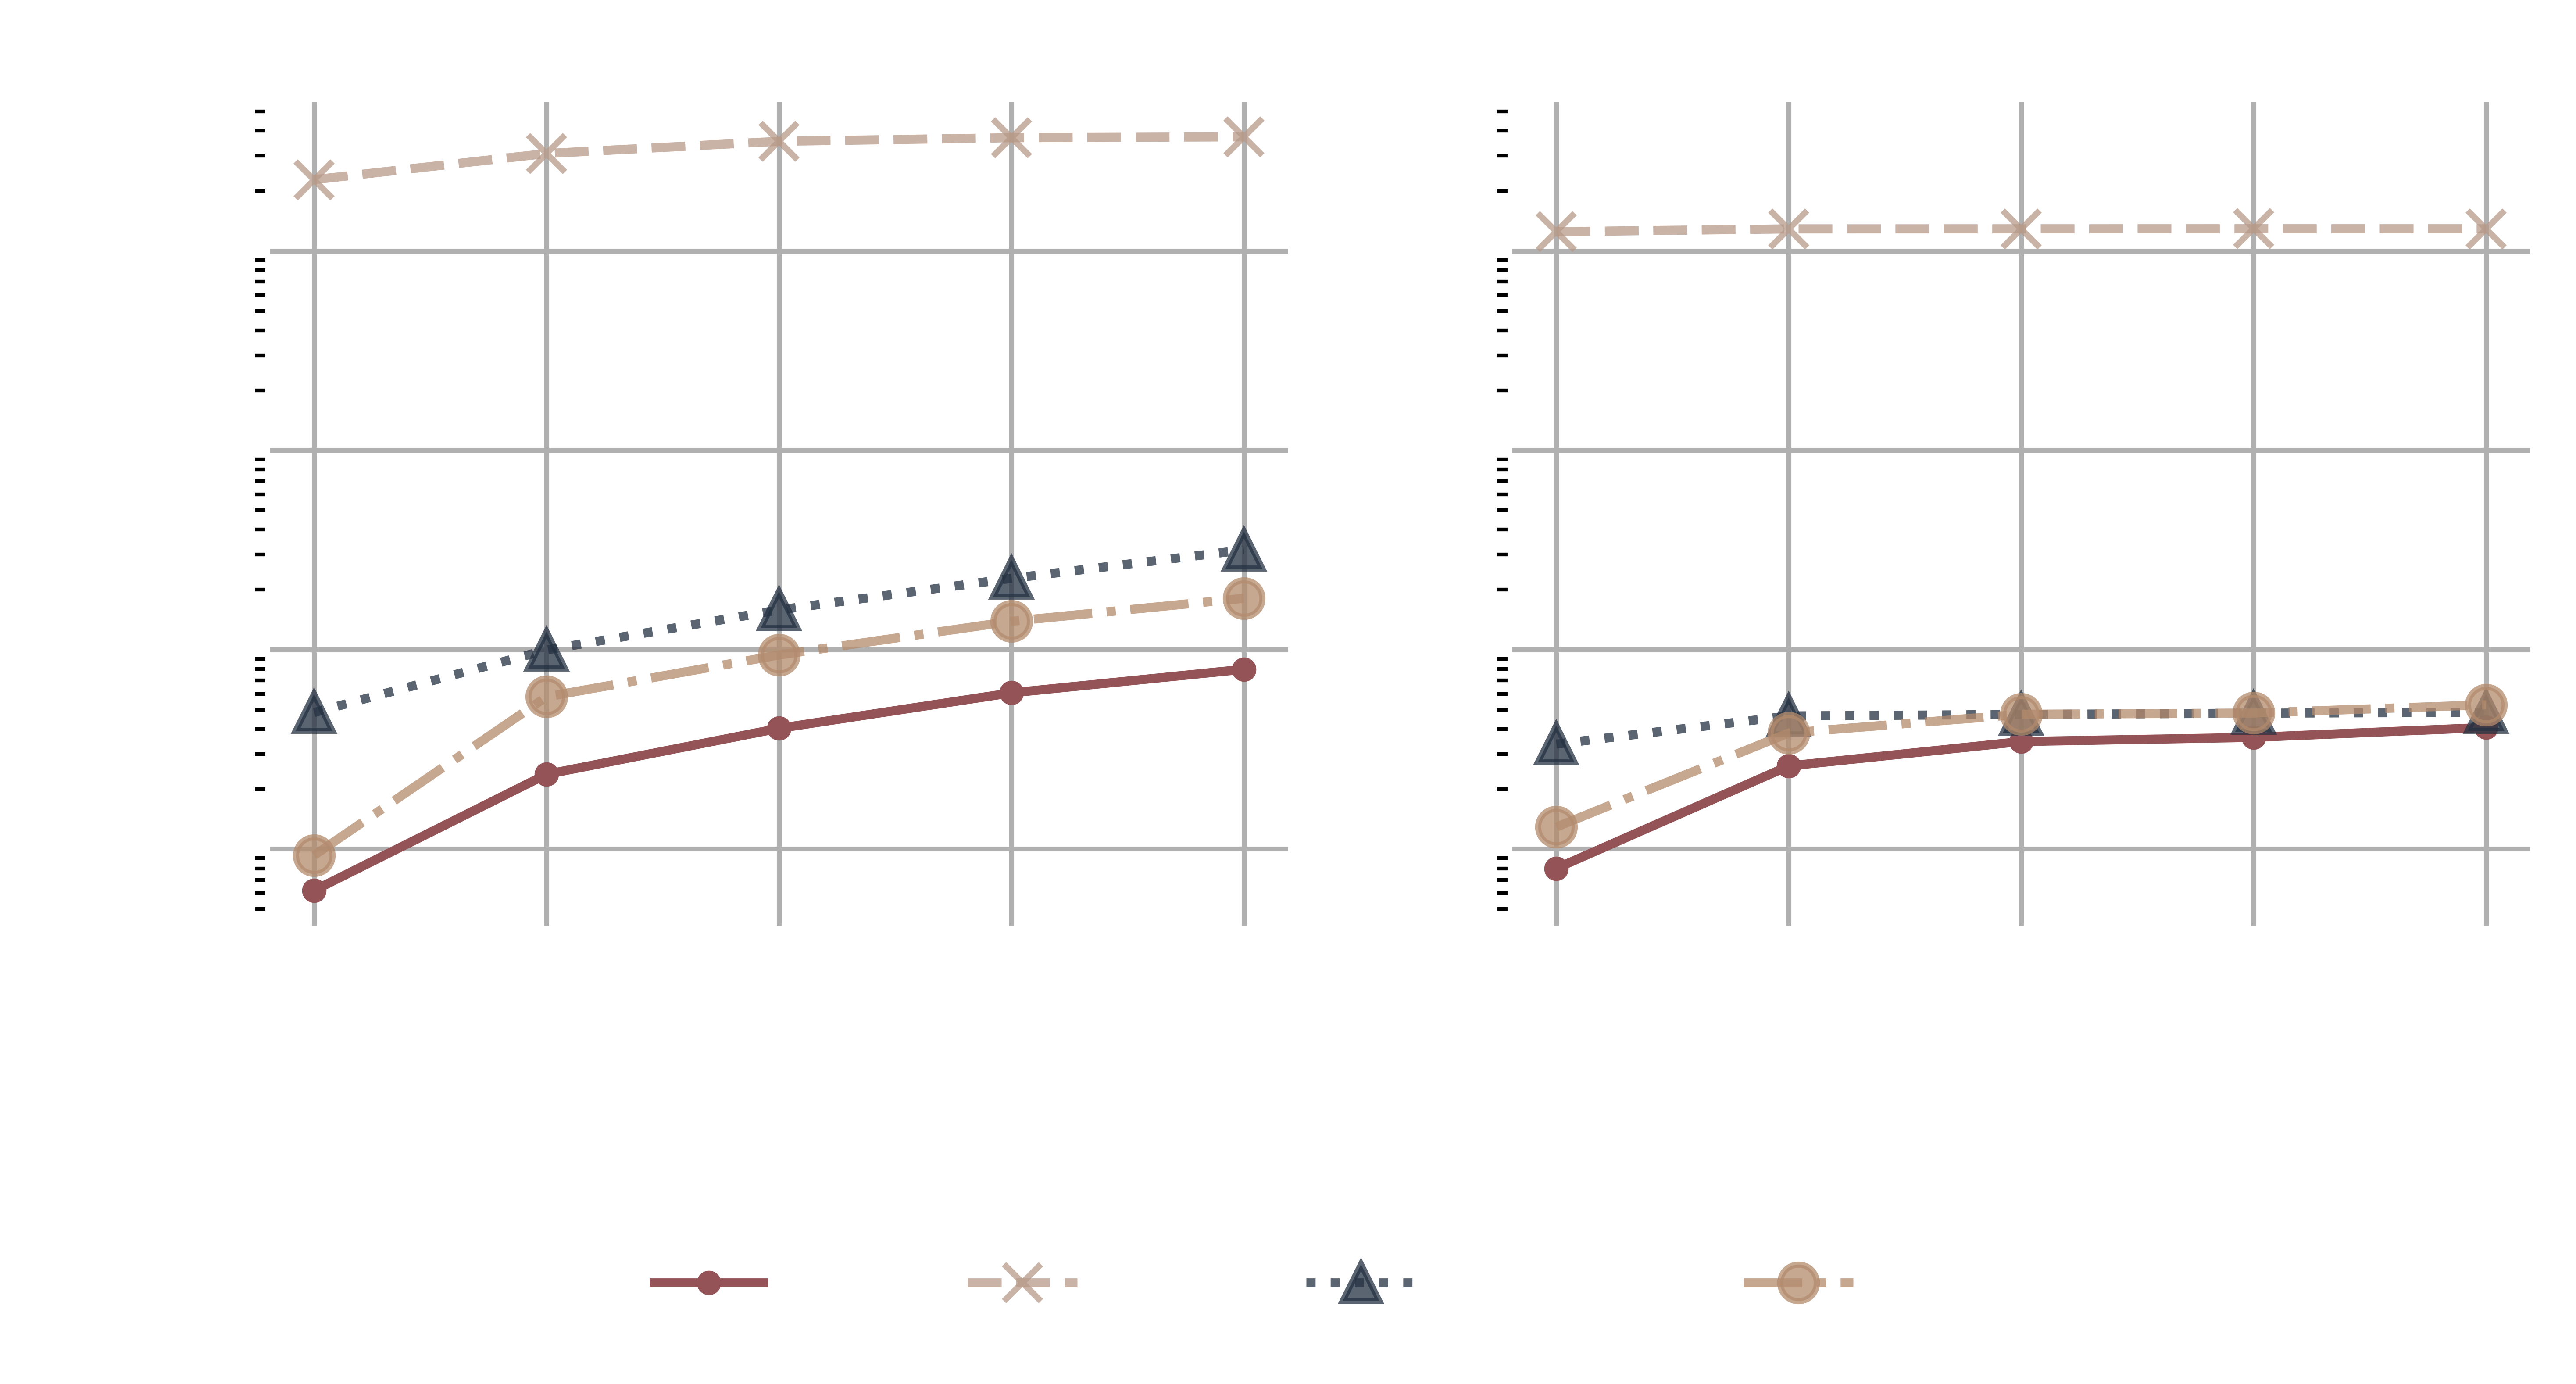
\includegraphics{absolute_performance_2-OAS-GDSW.pdf}
    \caption{Plot of the number of CG iterations $m$ required to achieve convergence of the solution to \cref{prob:elliptic_problem_discretized} in the sense of criterion \cref{eq:residual_convergence_criterion_r} with $\epsilon_r=10^{-8}$. The left and right columns correspons to the $\mathcal{C}_{\text{3layer, vert}}$ and $\mathcal{C}_{\text{edge slabs, around vertices}}$ coefficient functions. Also shown are the corresponding classical $m_1$, multi-cluster $m_{N_{\text{cluster}}}$, and multi-tail-cluster $m_{N_{\text{tail-cluster}}}$ bounds for the CG method applied to the eigenspectra obtained from the Lanczos matrix convergence (Ritz values).}
    \label{fig:cg_bounds_gdsw}
\end{figure}

\begin{figure}
    \centering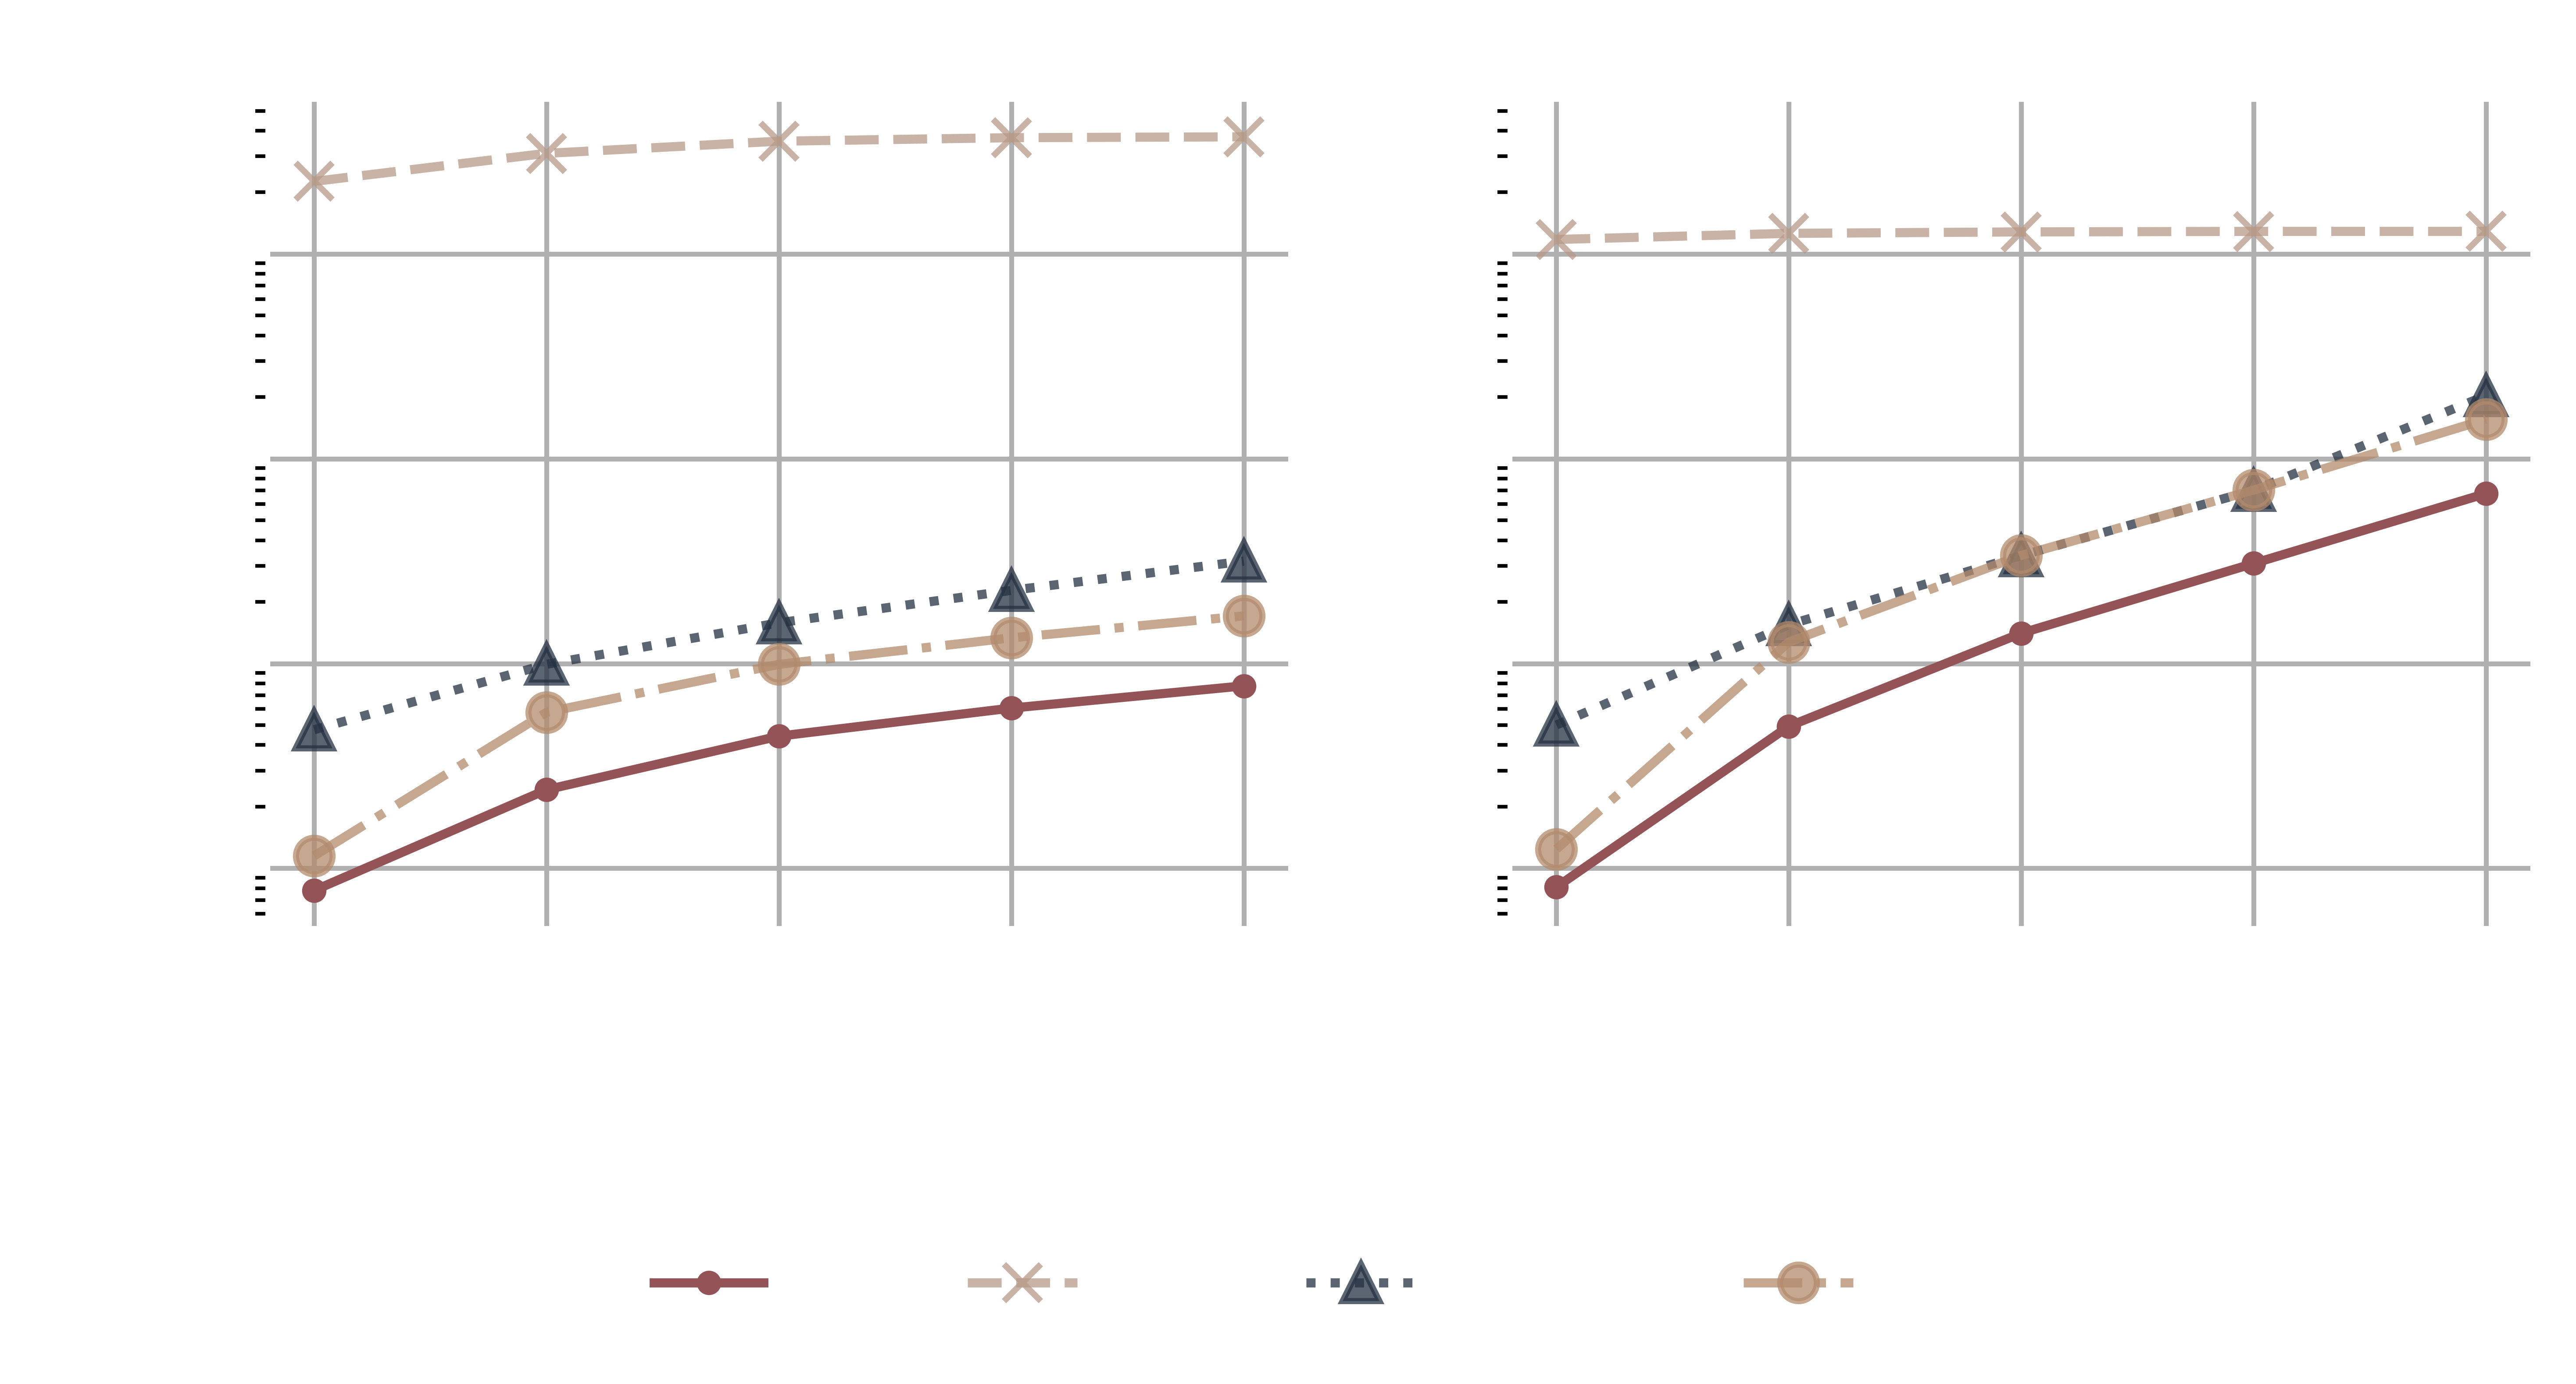
\includegraphics{absolute_performance_2-OAS-RGDSW.pdf}
    \caption{Similar to \cref{fig:cg_bounds_gdsw}, but now for RGDSW coarse space.}
    \label{fig:cg_bounds_rgdsw}
\end{figure}

\begin{figure}
    \centering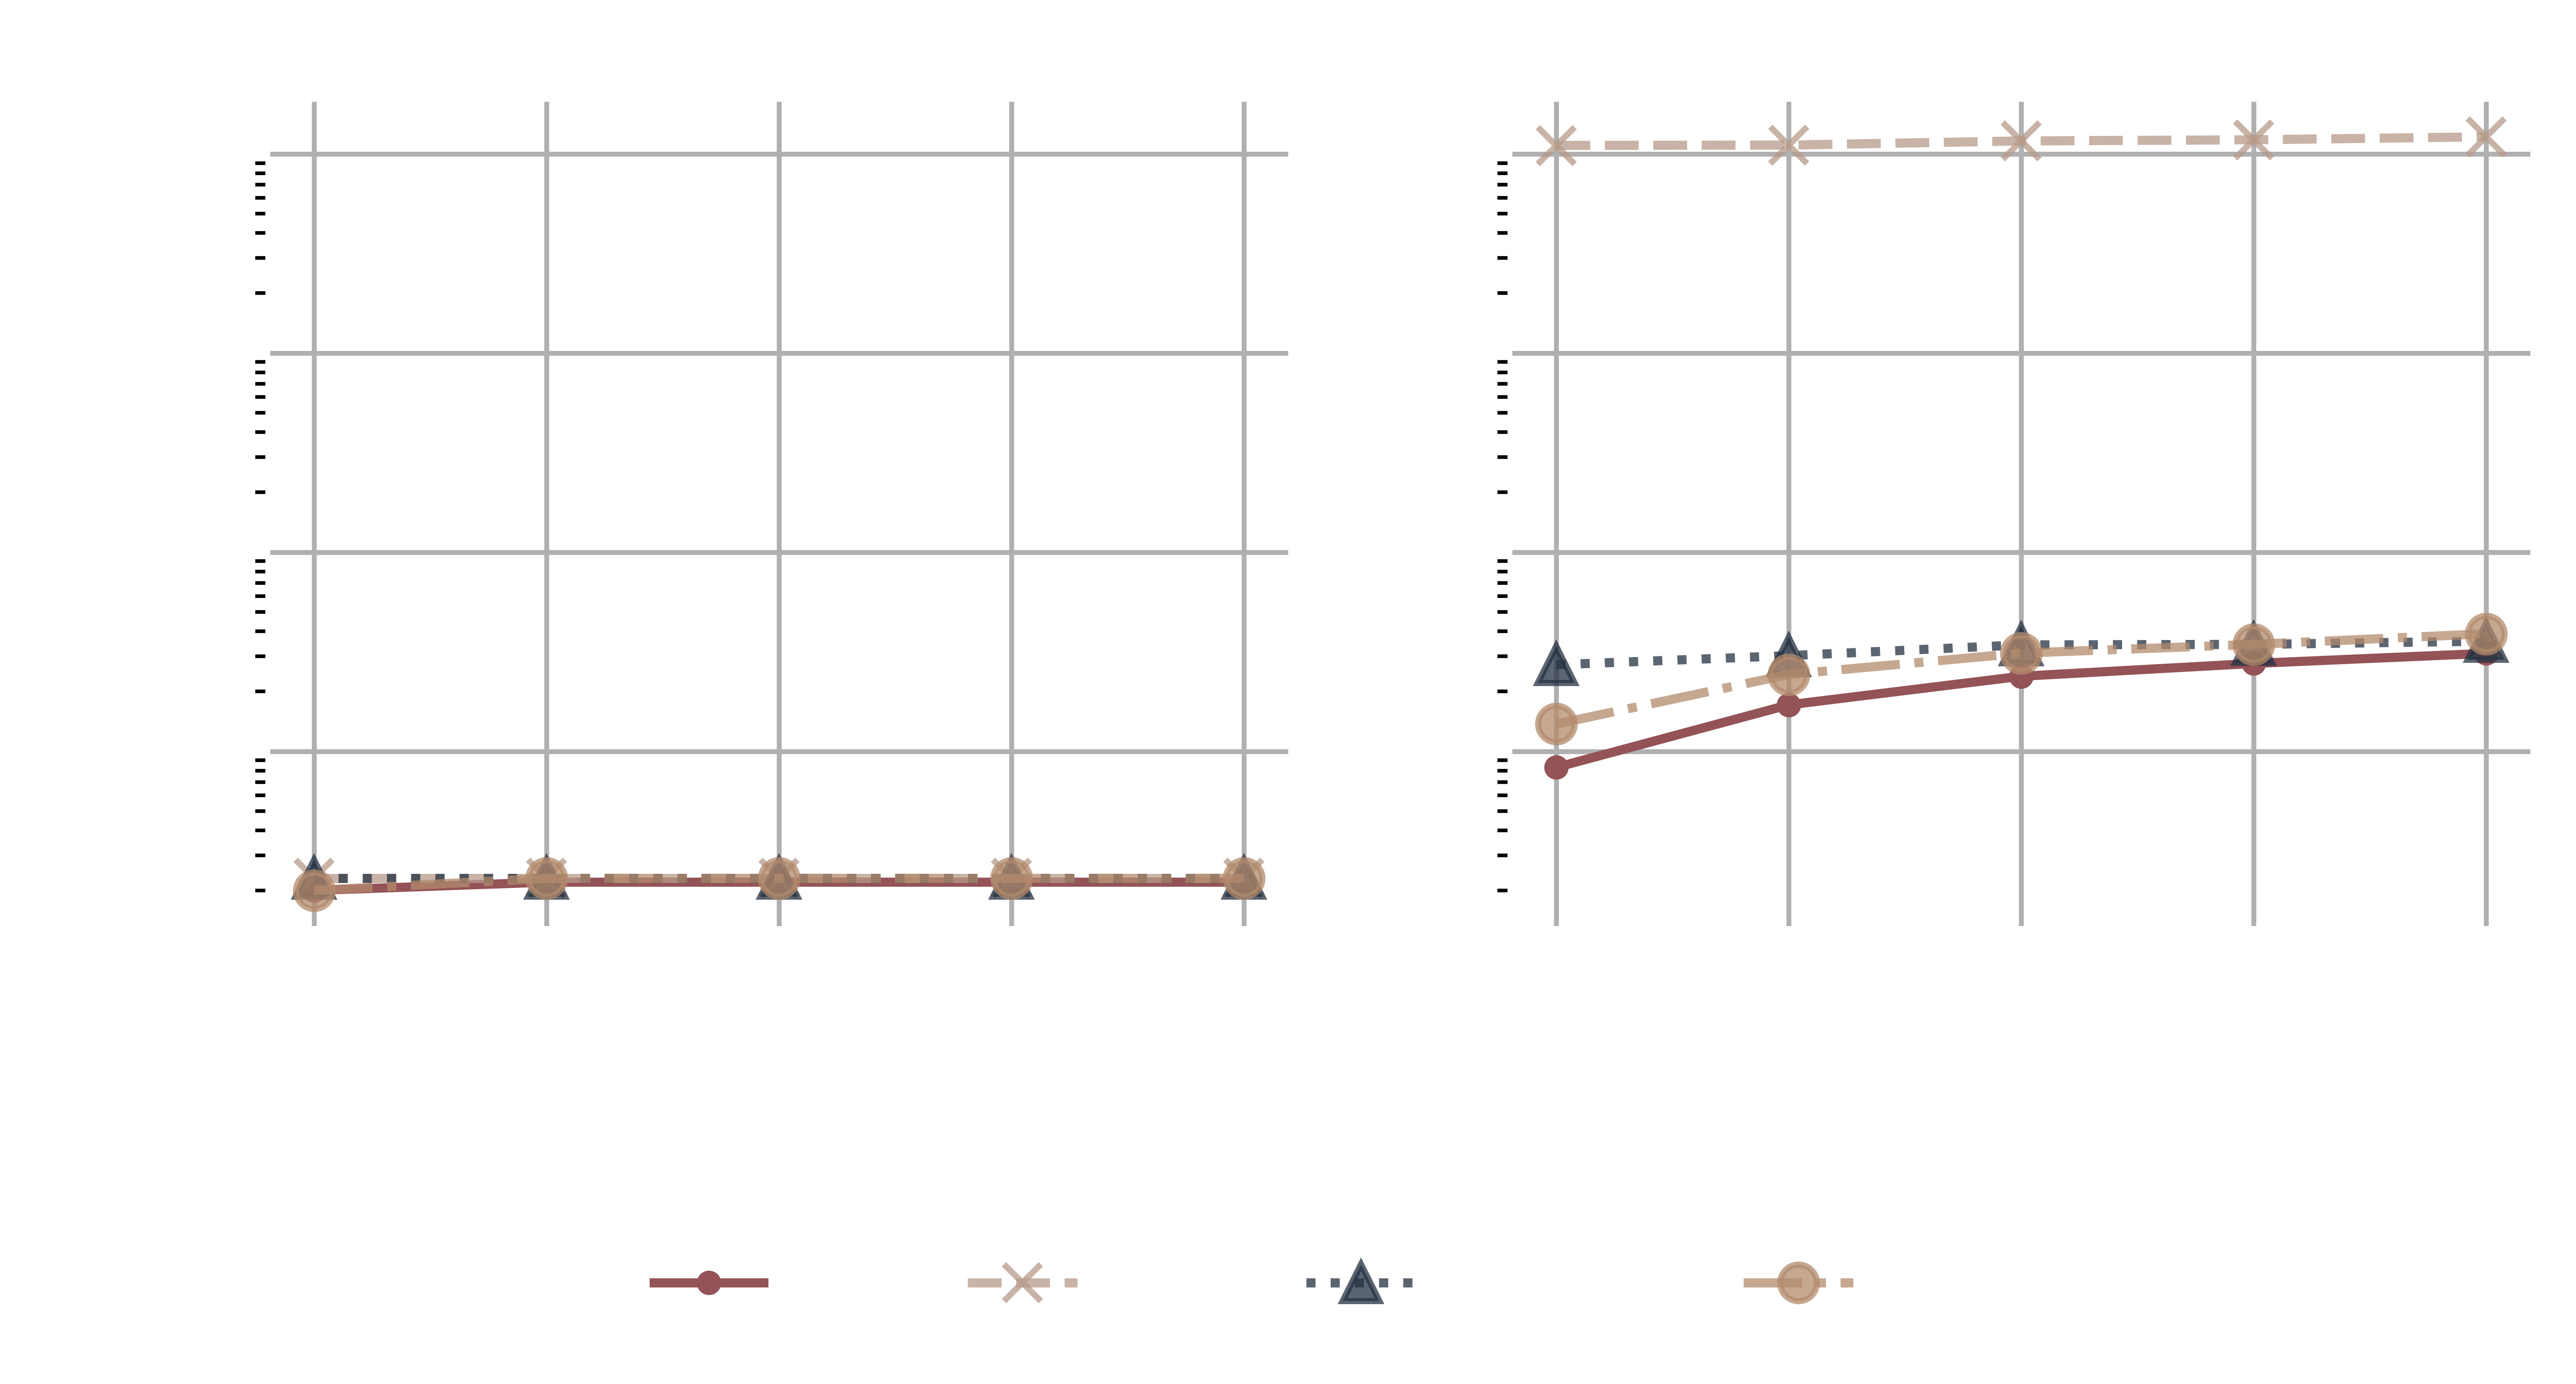
\includegraphics{absolute_performance_2-OAS-AMS.pdf}
    \caption{Similar to \cref{fig:cg_bounds_gdsw}, but now for AMS coarse space.}
    \label{fig:cg_bounds_ams}
\end{figure}

\section{Early estimation of CG iteration bounds}\label{sec:early_estimation_of_iterations}
\todo{Add plot of bounds convergence on some high-contrast coefficient function for a robust coarse space (AMS) together with its eigenspectrum. Explain the migration of Ritz values and the fact that we need to wait for temporary convergence of clusters to reliably calculate and update the new bounds.}
\todo{Show the convergence of the RGDSW bound. Ritz value migration happens more slowly so we need more iterations before we can update the bounds.}
\todo{Explain setup of tables}
\begin{table}[H]
\centering
\caption{PCG iteration bounds for solving the model diffusion problem with coefficient function $\mathcal{C}_{\mathrm{const}}$. Bounds are based on approximate spectra (Ritz values) obtained during the initial PCG iterations and are show for meshes $H=1/4$, $H=1/8$, $H=1/16$, $H=1/32$, $H=1/64$ and 2-OAS preconditioners with GDSW, RGDSW, AMS coarse spaces. The $\textbf{bound}$ columns show the values of the CG iteration bounds $m_1$, $m_{N_{\text{cluster}}}$, $m_{N_{\text{tail-cluster}}}$, $m_{\text{estimate}}$ and the $\textbf{iter.}$ columns show the iteration at which those bounds are obtained.}
\label{tab:cg_iteration_bound_coef=const}
\begin{tabular}{llrrrllrrll}
\toprule
 &  & \bfseries $m$ & \multicolumn{2}{|c|}{\bfseries $m_1$} & \multicolumn{2}{|c|}{\bfseries $m_{N_{\text{cluster}}}$} & \multicolumn{2}{|c|}{\bfseries $m_{N_{\text{tail-cluster}}}$} & \multicolumn{2}{|c|}{\bfseries $m_{\text{estimate}}$} \\
 &  &  & bound & iter. & bound & iter. & bound & iter. & bound & iter. \\
\midrule
\multirow[c]{3}{*}{\bfseries $H=1/4$} & GDSW & 23 & {\cellcolor[HTML]{004529}} \color[HTML]{F1F1F1} 34 & 11 & {\cellcolor[HTML]{BCE395}} \color[HTML]{000000} {\cellcolor[HTML]{ADD8E6}} - & - & {\cellcolor[HTML]{379E54}} \color[HTML]{F1F1F1} 34 & 11 & {\cellcolor[HTML]{FFFFE5}} \color[HTML]{000000} {\cellcolor[HTML]{ADD8E6}} - & - \\
\cline{2-11}
\bfseries  & RGDSW & 21 & {\cellcolor[HTML]{BCE395}} \color[HTML]{000000} 40 & 11 & {\cellcolor[HTML]{004529}} \color[HTML]{F1F1F1} {\cellcolor[HTML]{ADD8E6}} - & - & {\cellcolor[HTML]{379E54}} \color[HTML]{F1F1F1} 25 & 11 & {\cellcolor[HTML]{FFFFE5}} \color[HTML]{000000} {\cellcolor[HTML]{ADD8E6}} - & - \\
\cline{2-11}
\bfseries  & AMS & 18 & {\cellcolor[HTML]{BCE395}} \color[HTML]{000000} 23 & 11 & {\cellcolor[HTML]{004529}} \color[HTML]{F1F1F1} {\cellcolor[HTML]{ADD8E6}} - & - & {\cellcolor[HTML]{379E54}} \color[HTML]{F1F1F1} 20 & 11 & {\cellcolor[HTML]{FFFFE5}} \color[HTML]{000000} {\cellcolor[HTML]{ADD8E6}} - & - \\
\cline{1-11} \cline{2-11}
\multirow[c]{3}{*}{\bfseries $H=1/8$} & GDSW & 30 & {\cellcolor[HTML]{BCE395}} \color[HTML]{000000} 37 & 16 & {\cellcolor[HTML]{004529}} \color[HTML]{F1F1F1} {\cellcolor[HTML]{ADD8E6}} - & - & {\cellcolor[HTML]{379E54}} \color[HTML]{F1F1F1} 32 & 16 & {\cellcolor[HTML]{FFFFE5}} \color[HTML]{000000} {\cellcolor[HTML]{ADD8E6}} - & - \\
\cline{2-11}
\bfseries  & RGDSW & 32 & {\cellcolor[HTML]{004529}} \color[HTML]{F1F1F1} 43 & 11 & {\cellcolor[HTML]{BCE395}} \color[HTML]{000000} {\cellcolor[HTML]{ADD8E6}} - & - & {\cellcolor[HTML]{379E54}} \color[HTML]{F1F1F1} 43 & 11 & {\cellcolor[HTML]{FFFFE5}} \color[HTML]{000000} {\cellcolor[HTML]{ADD8E6}} - & - \\
\cline{2-11}
\bfseries  & AMS & 21 & {\cellcolor[HTML]{004529}} \color[HTML]{F1F1F1} 23 & 11 & {\cellcolor[HTML]{BCE395}} \color[HTML]{000000} {\cellcolor[HTML]{ADD8E6}} - & - & {\cellcolor[HTML]{379E54}} \color[HTML]{F1F1F1} 23 & 11 & {\cellcolor[HTML]{FFFFE5}} \color[HTML]{000000} {\cellcolor[HTML]{ADD8E6}} - & - \\
\cline{1-11} \cline{2-11}
\multirow[c]{3}{*}{\bfseries $H=1/16$} & GDSW & 33 & {\cellcolor[HTML]{BCE395}} \color[HTML]{000000} 37 & 16 & {\cellcolor[HTML]{004529}} \color[HTML]{F1F1F1} {\cellcolor[HTML]{ADD8E6}} - & - & {\cellcolor[HTML]{379E54}} \color[HTML]{F1F1F1} 32 & 16 & {\cellcolor[HTML]{FFFFE5}} \color[HTML]{000000} {\cellcolor[HTML]{ADD8E6}} - & - \\
\cline{2-11}
\bfseries  & RGDSW & 38 & {\cellcolor[HTML]{004529}} \color[HTML]{F1F1F1} 45 & 16 & {\cellcolor[HTML]{BCE395}} \color[HTML]{000000} {\cellcolor[HTML]{ADD8E6}} - & - & {\cellcolor[HTML]{379E54}} \color[HTML]{F1F1F1} 28 & 16 & {\cellcolor[HTML]{FFFFE5}} \color[HTML]{000000} {\cellcolor[HTML]{ADD8E6}} - & - \\
\cline{2-11}
\bfseries  & AMS & 22 & {\cellcolor[HTML]{004529}} \color[HTML]{F1F1F1} 24 & 16 & {\cellcolor[HTML]{BCE395}} \color[HTML]{000000} {\cellcolor[HTML]{ADD8E6}} - & - & {\cellcolor[HTML]{379E54}} \color[HTML]{F1F1F1} 24 & 16 & {\cellcolor[HTML]{FFFFE5}} \color[HTML]{000000} {\cellcolor[HTML]{ADD8E6}} - & - \\
\cline{1-11} \cline{2-11}
\multirow[c]{3}{*}{\bfseries $H=1/32$} & GDSW & 35 & {\cellcolor[HTML]{004529}} \color[HTML]{F1F1F1} 37 & 16 & {\cellcolor[HTML]{BCE395}} \color[HTML]{000000} {\cellcolor[HTML]{ADD8E6}} - & - & {\cellcolor[HTML]{379E54}} \color[HTML]{F1F1F1} 28 & 16 & {\cellcolor[HTML]{FFFFE5}} \color[HTML]{000000} {\cellcolor[HTML]{ADD8E6}} - & - \\
\cline{2-11}
\bfseries  & RGDSW & 42 & {\cellcolor[HTML]{004529}} \color[HTML]{F1F1F1} 44 & 16 & {\cellcolor[HTML]{BCE395}} \color[HTML]{000000} {\cellcolor[HTML]{ADD8E6}} - & - & {\cellcolor[HTML]{379E54}} \color[HTML]{F1F1F1} 28 & 16 & {\cellcolor[HTML]{FFFFE5}} \color[HTML]{000000} {\cellcolor[HTML]{ADD8E6}} - & - \\
\cline{2-11}
\bfseries  & AMS & 22 & {\cellcolor[HTML]{004529}} \color[HTML]{F1F1F1} 24 & 16 & {\cellcolor[HTML]{BCE395}} \color[HTML]{000000} {\cellcolor[HTML]{ADD8E6}} - & - & {\cellcolor[HTML]{379E54}} \color[HTML]{F1F1F1} 24 & 16 & {\cellcolor[HTML]{FFFFE5}} \color[HTML]{000000} {\cellcolor[HTML]{ADD8E6}} - & - \\
\cline{1-11} \cline{2-11}
\multirow[c]{3}{*}{\bfseries $H=1/64$} & GDSW & 36 & {\cellcolor[HTML]{004529}} \color[HTML]{F1F1F1} 37 & 16 & {\cellcolor[HTML]{BCE395}} \color[HTML]{000000} {\cellcolor[HTML]{ADD8E6}} - & - & {\cellcolor[HTML]{379E54}} \color[HTML]{F1F1F1} 28 & 16 & {\cellcolor[HTML]{FFFFE5}} \color[HTML]{000000} {\cellcolor[HTML]{ADD8E6}} - & - \\
\cline{2-11}
\bfseries  & RGDSW & 45 & {\cellcolor[HTML]{004529}} \color[HTML]{F1F1F1} 44 & 16 & {\cellcolor[HTML]{BCE395}} \color[HTML]{000000} {\cellcolor[HTML]{ADD8E6}} - & - & {\cellcolor[HTML]{379E54}} \color[HTML]{F1F1F1} 36 & 16 & {\cellcolor[HTML]{FFFFE5}} \color[HTML]{000000} {\cellcolor[HTML]{ADD8E6}} - & - \\
\cline{2-11}
\bfseries  & AMS & 23 & {\cellcolor[HTML]{004529}} \color[HTML]{F1F1F1} 29 & 11 & {\cellcolor[HTML]{BCE395}} \color[HTML]{000000} {\cellcolor[HTML]{ADD8E6}} - & - & {\cellcolor[HTML]{379E54}} \color[HTML]{F1F1F1} 29 & 11 & {\cellcolor[HTML]{FFFFE5}} \color[HTML]{000000} {\cellcolor[HTML]{ADD8E6}} - & - \\
\cline{1-11} \cline{2-11}
\bottomrule
\end{tabular}
\end{table}

\begin{table}[H]
\centering
\caption{PCG iteration bounds $m_1$, $m_{N_{\text{cluster}}}$, $m_{N_{\text{tail-cluster}}}$, $m_{\text{estimate}}$ for solving the model diffusion problem with coefficient function $\mathcal{C}_{\mathrm{3layer, \ vert}}$. Bounds are based on approximate spectra (Ritz values) obtained during the initial PCG iterations and are shown for meshes $\mathbf{H=1/4}$, $\mathbf{H=1/8}$, $\mathbf{H=1/16}$, $\mathbf{H=1/32}$, $\mathbf{H=1/64}$ and 2-OAS preconditioners with GDSW, RGDSW, AMS coarse spaces. The $\textbf{iter.}$ column shows the iteration at which the bounds are obtained.}
\label{tab:cg_iteration_bound_coef=3lvert}
\begin{tabular}{llrrrrrr}
\toprule
 &  & $m$ & $m_1$ & $m_{N_{\text{cluster}}}$ & $m_{N_{\text{tail-cluster}}}$ & $m_{\text{estimate}}$ & \textbf{iter.} \\
\midrule
\multirow[c]{3}{*}{$\mathbf{H=1/4}$} & GDSW & 62 & {\cellcolor[HTML]{E2E4FB}} \color[HTML]{000000} 225,419 & {\cellcolor[HTML]{ACB8F4}} \color[HTML]{000000} 111 & {\cellcolor[HTML]{768BEC}} \color[HTML]{F1F1F1} 26 & {\cellcolor[HTML]{405FE5}} \color[HTML]{F1F1F1} 69 & 26 \\
\cline{2-8}
 & RGDSW & 78 & {\cellcolor[HTML]{E2E4FB}} \color[HTML]{000000} 224,028 & {\cellcolor[HTML]{768BEC}} \color[HTML]{F1F1F1} 109 & {\cellcolor[HTML]{ACB8F4}} \color[HTML]{000000} 26 & {\cellcolor[HTML]{405FE5}} \color[HTML]{F1F1F1} 68 & 26 \\
\cline{2-8}
 & AMS & 20 & {\cellcolor[HTML]{405FE5}} \color[HTML]{F1F1F1} 23 & {\cellcolor[HTML]{405FE5}} \color[HTML]{F1F1F1} 23 & {\cellcolor[HTML]{E2E4FB}} \color[HTML]{000000} 11 & {\cellcolor[HTML]{405FE5}} \color[HTML]{F1F1F1} 17 & 11 \\
\cline{1-8} \cline{2-8}
\multirow[c]{3}{*}{$\mathbf{H=1/8}$} & GDSW & 237 & {\cellcolor[HTML]{E2E4FB}} \color[HTML]{000000} 300,788 & {\cellcolor[HTML]{ACB8F4}} \color[HTML]{000000} 641 & {\cellcolor[HTML]{768BEC}} \color[HTML]{F1F1F1} 91 & {\cellcolor[HTML]{405FE5}} \color[HTML]{F1F1F1} 366 & 51 \\
\cline{2-8}
 & RGDSW & 242 & {\cellcolor[HTML]{E2E4FB}} \color[HTML]{000000} 302,967 & {\cellcolor[HTML]{ACB8F4}} \color[HTML]{000000} 638 & {\cellcolor[HTML]{768BEC}} \color[HTML]{F1F1F1} 86 & {\cellcolor[HTML]{405FE5}} \color[HTML]{F1F1F1} 362 & 51 \\
\cline{2-8}
 & AMS & 22 & {\cellcolor[HTML]{405FE5}} \color[HTML]{F1F1F1} 23 & {\cellcolor[HTML]{405FE5}} \color[HTML]{F1F1F1} 23 & {\cellcolor[HTML]{E2E4FB}} \color[HTML]{000000} 11 & {\cellcolor[HTML]{91A1F0}} \color[HTML]{F1F1F1} 17 & 11 \\
\cline{1-8} \cline{2-8}
\multirow[c]{3}{*}{$\mathbf{H=1/16}$} & GDSW & 403 & {\cellcolor[HTML]{E2E4FB}} \color[HTML]{000000} 350,992 & {\cellcolor[HTML]{ACB8F4}} \color[HTML]{000000} 949 & {\cellcolor[HTML]{768BEC}} \color[HTML]{F1F1F1} 148 & {\cellcolor[HTML]{405FE5}} \color[HTML]{F1F1F1} 549 & 96 \\
\cline{2-8}
 & RGDSW & 442 & {\cellcolor[HTML]{E2E4FB}} \color[HTML]{000000} 351,891 & {\cellcolor[HTML]{ACB8F4}} \color[HTML]{000000} 948 & {\cellcolor[HTML]{768BEC}} \color[HTML]{F1F1F1} 147 & {\cellcolor[HTML]{405FE5}} \color[HTML]{F1F1F1} 548 & 96 \\
\cline{2-8}
 & AMS & 22 & {\cellcolor[HTML]{405FE5}} \color[HTML]{F1F1F1} 23 & {\cellcolor[HTML]{405FE5}} \color[HTML]{F1F1F1} 23 & {\cellcolor[HTML]{E2E4FB}} \color[HTML]{000000} 11 & {\cellcolor[HTML]{91A1F0}} \color[HTML]{F1F1F1} 17 & 11 \\
\cline{1-8} \cline{2-8}
\multirow[c]{3}{*}{$\mathbf{H=1/32}$} & GDSW & 607 & {\cellcolor[HTML]{E2E4FB}} \color[HTML]{000000} 367,021 & {\cellcolor[HTML]{ACB8F4}} \color[HTML]{000000} 2,228 & {\cellcolor[HTML]{405FE5}} \color[HTML]{F1F1F1} 231 & {\cellcolor[HTML]{768BEC}} \color[HTML]{F1F1F1} 1,230 & 161 \\
\cline{2-8}
 & RGDSW & 606 & {\cellcolor[HTML]{E2E4FB}} \color[HTML]{000000} 368,220 & {\cellcolor[HTML]{ACB8F4}} \color[HTML]{000000} 2,277 & {\cellcolor[HTML]{405FE5}} \color[HTML]{F1F1F1} 290 & {\cellcolor[HTML]{768BEC}} \color[HTML]{F1F1F1} 1,284 & 216 \\
\cline{2-8}
 & AMS & 22 & {\cellcolor[HTML]{405FE5}} \color[HTML]{F1F1F1} 23 & {\cellcolor[HTML]{405FE5}} \color[HTML]{F1F1F1} 23 & {\cellcolor[HTML]{E2E4FB}} \color[HTML]{000000} 11 & {\cellcolor[HTML]{91A1F0}} \color[HTML]{F1F1F1} 17 & 11 \\
\cline{1-8} \cline{2-8}
\multirow[c]{3}{*}{$\mathbf{H=1/64}$} & GDSW & 797 & {\cellcolor[HTML]{E2E4FB}} \color[HTML]{000000} 359,087 & {\cellcolor[HTML]{ACB8F4}} \color[HTML]{000000} 1,764 & {\cellcolor[HTML]{768BEC}} \color[HTML]{F1F1F1} 85 & {\cellcolor[HTML]{405FE5}} \color[HTML]{F1F1F1} 925 & 46 \\
\cline{2-8}
 & RGDSW & 778 & {\cellcolor[HTML]{E2E4FB}} \color[HTML]{000000} 359,976 & {\cellcolor[HTML]{ACB8F4}} \color[HTML]{000000} 1,763 & {\cellcolor[HTML]{768BEC}} \color[HTML]{F1F1F1} 85 & {\cellcolor[HTML]{405FE5}} \color[HTML]{F1F1F1} 924 & 51 \\
\cline{2-8}
 & AMS & 22 & {\cellcolor[HTML]{405FE5}} \color[HTML]{F1F1F1} 23 & {\cellcolor[HTML]{405FE5}} \color[HTML]{F1F1F1} 23 & {\cellcolor[HTML]{E2E4FB}} \color[HTML]{000000} 11 & {\cellcolor[HTML]{91A1F0}} \color[HTML]{F1F1F1} 17 & 11 \\
\cline{1-8} \cline{2-8}
\bottomrule
\end{tabular}
\end{table}

\begin{table}[H]
\centering
\caption{PCG iteration bounds for coefficient function $\mathcal{C}_{\mathrm{edge \ slabs, \ around \ vertices}}$ based on approximate spectra (Ritz values) from the first 300 iterations of solving the model diffusion problem on the meshes $H=1/4$, $H=1/8$, $H=1/16$, $H=1/32$, $H=1/64$ using 2-OAS preconditioners with GDSW, RGDSW, AMS coarse spaces. The $\textbf{bound}$ columns show the values of the CG iteration bounds $m_1$, $m_{N_{\text{cluster}}}$, $m_{N_{\text{tail-cluster}}}$, $m_{\text{estimate}}$ and the ($\textbf{iter.}$) column shows the iteration at which these are obtained.}
\label{tab:cg_iteration_bound_Nc64_N=300}
\begin{tabular}{llrrrrrrrrr}
\toprule
 &  & m & \multicolumn{2}{|c|}{$m_1$} & \multicolumn{2}{|c|}{$m_{N_{\text{cluster}}}$} & \multicolumn{2}{|c|}{$m_{N_{\text{tail-cluster}}}$} & \multicolumn{2}{|c|}{$m_{\text{estimate}}$} \\
 &  & \rotatebox{45}{\bfseries } & \rotatebox{45}{\bfseries bound} & \rotatebox{45}{\bfseries iter.} & \rotatebox{45}{\bfseries bound} & \rotatebox{45}{\bfseries iter.} & \rotatebox{45}{\bfseries bound} & \rotatebox{45}{\bfseries iter.} & \rotatebox{45}{\bfseries bound} & \rotatebox{45}{\bfseries iter.} \\
\midrule
\multirow[c]{3}{*}{$H=1/4$} & GDSW & 80 & 124,727 & 36 & 88 & 36 & 88 & 36 & 88 & 36 \\
 & RGDSW & 81 & 117,699 & 36 & 133 & 36 & 61 & 36 & 97 & 36 \\
 & AMS & 83 & 105,144 & 66 & 218 & 66 & 111 & 66 & 165 & 66 \\
\cline{1-11}
\multirow[c]{3}{*}{$H=1/8$} & GDSW & 261 & 127,648 & 96 & 383 & 96 & 173 & 96 & 278 & 96 \\
 & RGDSW & 494 & 124,745 & 186 & 1,274 & 186 & 583 & 186 & 929 & 186 \\
 & AMS & 171 & 110,677 & 71 & 302 & 71 & 123 & 71 & 213 & 71 \\
\cline{1-11}
\multirow[c]{3}{*}{$H=1/16$} & GDSW & 346 & 123,872 & 76 & 306 & 76 & 134 & 76 & 220 & 76 \\
 & RGDSW & 1,406 & 122,195 & 241 & 2,185 & 241 & 979 & 241 & 1,582 & 241 \\
 & AMS & 238 & 110,969 & 81 & 310 & 81 & 126 & 81 & 218 & 81 \\
\cline{1-11}
\multirow[c]{3}{*}{$H=1/32$} & GDSW & 363 & 122,634 & 76 & 310 & 76 & 136 & 76 & 223 & 76 \\
 & RGDSW & 3,082 & 109,007 & 271 & 1,415 & 271 & 920 & 271 & 1,168 & 271 \\
 & AMS & 276 & 116,797 & 191 & 344 & 191 & 251 & 191 & 298 & 191 \\
\cline{1-11}
\multirow[c]{3}{*}{$H=1/64$} & GDSW & 407 & 127,897 & 186 & 485 & 186 & 268 & 186 & 377 & 186 \\
 & RGDSW & 6,766 & 69,645 & 291 & 2,612 & 291 & 956 & 291 & 1,784 & 291 \\
 & AMS & 310 & 120,694 & 196 & 357 & 196 & 260 & 196 & 309 & 196 \\
\cline{1-11}
\bottomrule
\end{tabular}
\end{table}

\todo{Discuss the tables: how many iterations are needed to get a good estimate of the bounds? How do the bounds compare to the classical bound? How do the bounds compare to each other?}

\begin{frame}{Structure: Outlook}
    \frametitle{Structure}
    \begin{itemize}
        \item Research Questions
        \item Mathematical Background
        \item Related Work
        \item Preliminary Results
        \item {\color{tud grapefruit}Outlook}
    \end{itemize}
\end{frame}

\begin{frame}{Outlook: Q1}
    \frametitle{Outlook}
    \framesubtitle{Research Question 1 answered}
\end{frame}

\begin{frame}{Outlook: Q3}
    \frametitle{Outlook}
    \framesubtitle{Research question 3 answered}
\end{frame}

\begin{frame}{Outlook: Next steps}
    \frametitle{Outlook}
    \framesubtitle{Next steps}
    \begin{itemize}
        \item Work on answering research questions 4, 5, and 6.
    \end{itemize}
\end{frame}

\begin{frame}{Outlook: Open Challenge}
    \frametitle{Outlook}
    \framesubtitle{Open Challenge}
    \begin{itemize}
        \item How to answer research question 2?
    \end{itemize}
\end{frame}

\end{document}